% ----------------------------------------------------------------------
% Unofficial UCLA SCC Latex Beamer Presentation
% Author: Denise Ferrari  <denise@stat.ucla.edu>
% Date: 03/17/2009
% ----------------------------------------------------------------------
% This presentation requires the following files:
%
% beamerthemeSCC.sty
% beamerouterthemeSCC.sty
% beamercolorthemeSCC.sty
% logo.png
% ----------------------------------------------------------------------
% ----------------------------------------------------------------------

\documentclass[11pt]{beamer}

%% To get handouts:
% \documentclass[11pt,containsverbatim,handout]{beamer}

%% include when making handouts
% \usepackage{pgfpages}
% \pgfpagesuselayout{4 on 1}[letterpaper,landscape,border shrink=5mm]

% *****************************************
% Theme
% *****************************************

% use compress for circles to be on one line
% o/w take it out
% \usetheme{SCC}
\usetheme[compress]{SCC}

% *****************************************
% Packages
% *****************************************
\usepackage{graphicx}
\usepackage{amssymb}
\usepackage{epstopdf}
\usepackage{listings}
\usepackage{hyperref}
\usepackage{color}

\DeclareGraphicsRule{.tif}{png}{.png}{`convert #1 `dirname #1`/`basename #1 .tif`.png}

\lstloadlanguages{R} 
\lstset{language=R,%
basicstyle=\small\ttfamily,%
stringstyle=\color{magenta},%
showstringspaces=false,%
keywordstyle=\color{red}\mdseries\underbar,%
commentstyle=\color{green}\textsl,%
xleftmargin=4ex,%
numbers=left,%
numberstyle=\tiny,%
stepnumber=1,%
firstnumber=1,%
breaklines=true%
}

% *****************************************
% New Commands
% *****************************************
\newcommand{\urlwofont}[1]
{
\urlstyle{same}\url{#1}
}

% Presentation

\begin{document}
	% Title
% Note: [short title]{long title}, [short author(s) name]{long author(s) name}
\title{ \ttfamily R \normalfont Graphics II: Graphics for Exploratory Data Analysis}
%\subtitle{}
\author{Irina Kukuyeva \\ \ttfamily ikukuyeva@stat.ucla.edu \normalfont}
\institute[UCLA SCC]{UCLA Extension Track 1\\UCLA Department of Statistics \\ Statistical Consulting Center}
\date{January 12, 2011}



% Title Frame 
\frame{ \titlepage }

	% TOC
\begin{frame}[shrink=6]
	\frametitle{Outline}
	\tableofcontents[hideallsubsections]
\end{frame}

% Before any section, show a slide that highlights the current section 
\AtBeginSection[]
{
	\begin{frame} [shrink=6]
		\tableofcontents[currentsection,hideothersubsections]
	\end{frame}
}
	%%%%%%%%%%%%%%%%%%%%%%%%%%%%%%%%%%%%%
\part{Preliminaries}
%%%%%%%%%%%%%%%%%%%%%%%%%%%%%%%%%%%%%

%%% --------------------------
\section{Motivation}
\subsection{Why tutorial?} 
%%% --------------------------
\normalfont
\begin{frame}
	\begin{center}
  		\begin{alertblock}{Why Tutorial?} 
  			\begin{itemize}
  				\item Derive and convey key insights from data
  				\item Learn and use open source software
  				\item Explore first/another programming language
  				\item Gain ability to create insightful visualizations
  				\item Be more marketable 
  			\end{itemize}
		\end{alertblock}

	       \begin{center}
	         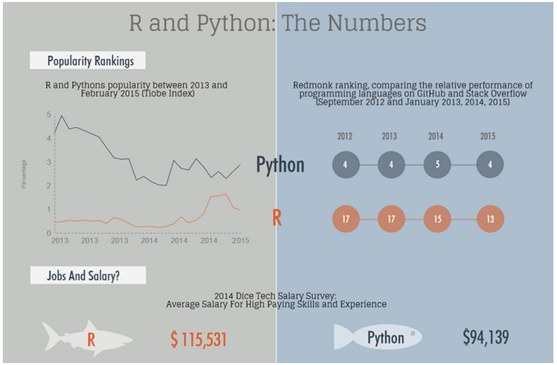
\includegraphics[scale=0.25]{images/r-vs-python-numbers}[6]
	        \end{center}

	\end{center} 
\end{frame}


%%% --------------------------
\subsection{Why R?}
%%% --------------------------
\begin{frame}
	\begin{center}
  		\begin{block}{Why R?} 
			\begin{itemize}
				\item Absolutely free!
				\item Used in industry and academia.
				\item Has a great community:
					\begin{itemize}
						\item StackOverflow
						\item Blogs
						\item Meetup groups
						\item MOOCs
						\item many, many others
					\end{itemize}
				\item Has over 7900 packages available for use (for free!).
				\item Transparent code (e.g. easier to check for bugs).
			\end{itemize}
		\end{block}
	\end{center} 
\end{frame}

%%% --------------------------
\subsection{Why visualize?}
%%% --------------------------
\begin{frame}
	\frametitle{Approach 1: Infographic}
	\begin{center}
		\vspace{-10pt}
  		\begin{block}{Inforgraphic} 
			\begin{itemize}
				\item Manually created
				\item Customized to a data set
				\item Art
			\end{itemize}
		\end{block}
	\end{center}	

   \begin{center}
     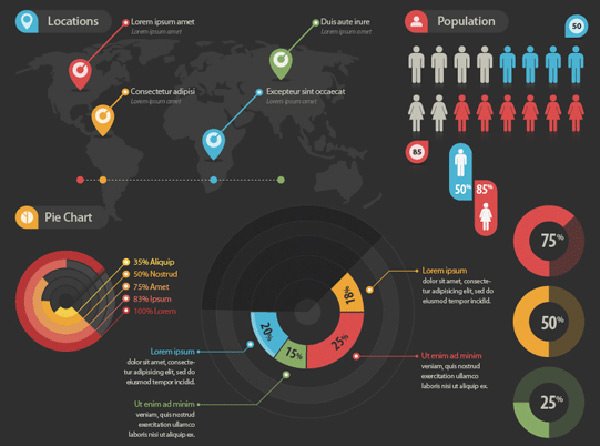
\includegraphics[scale=0.25]{images/infographic}[10]
    \end{center}

\end{frame}


\begin{frame}[allowframebreaks]
	\frametitle{Approach 2: Data Visualization}
  		\begin{block}{Data Visualization} 
			\begin{itemize}
				\item Automated via software
				\item Reproducible for a different data set
				\item (Less? of an) art
			\end{itemize}
		\end{block}
		There are two types of data visualization:
			\begin{block}{1. Exploratory} 
					\begin{itemize}
						\item \small Capture uncertainty in the data
						\item Explore potential relationships/trends/missing patterns (or absence thereof)
					\end{itemize}
			\end{block}
			\begin{block}{2. Explanatory}
					\begin{itemize}
						\item Convey key information \normalfont
					\end{itemize}
			\end{block}

   \begin{center}
     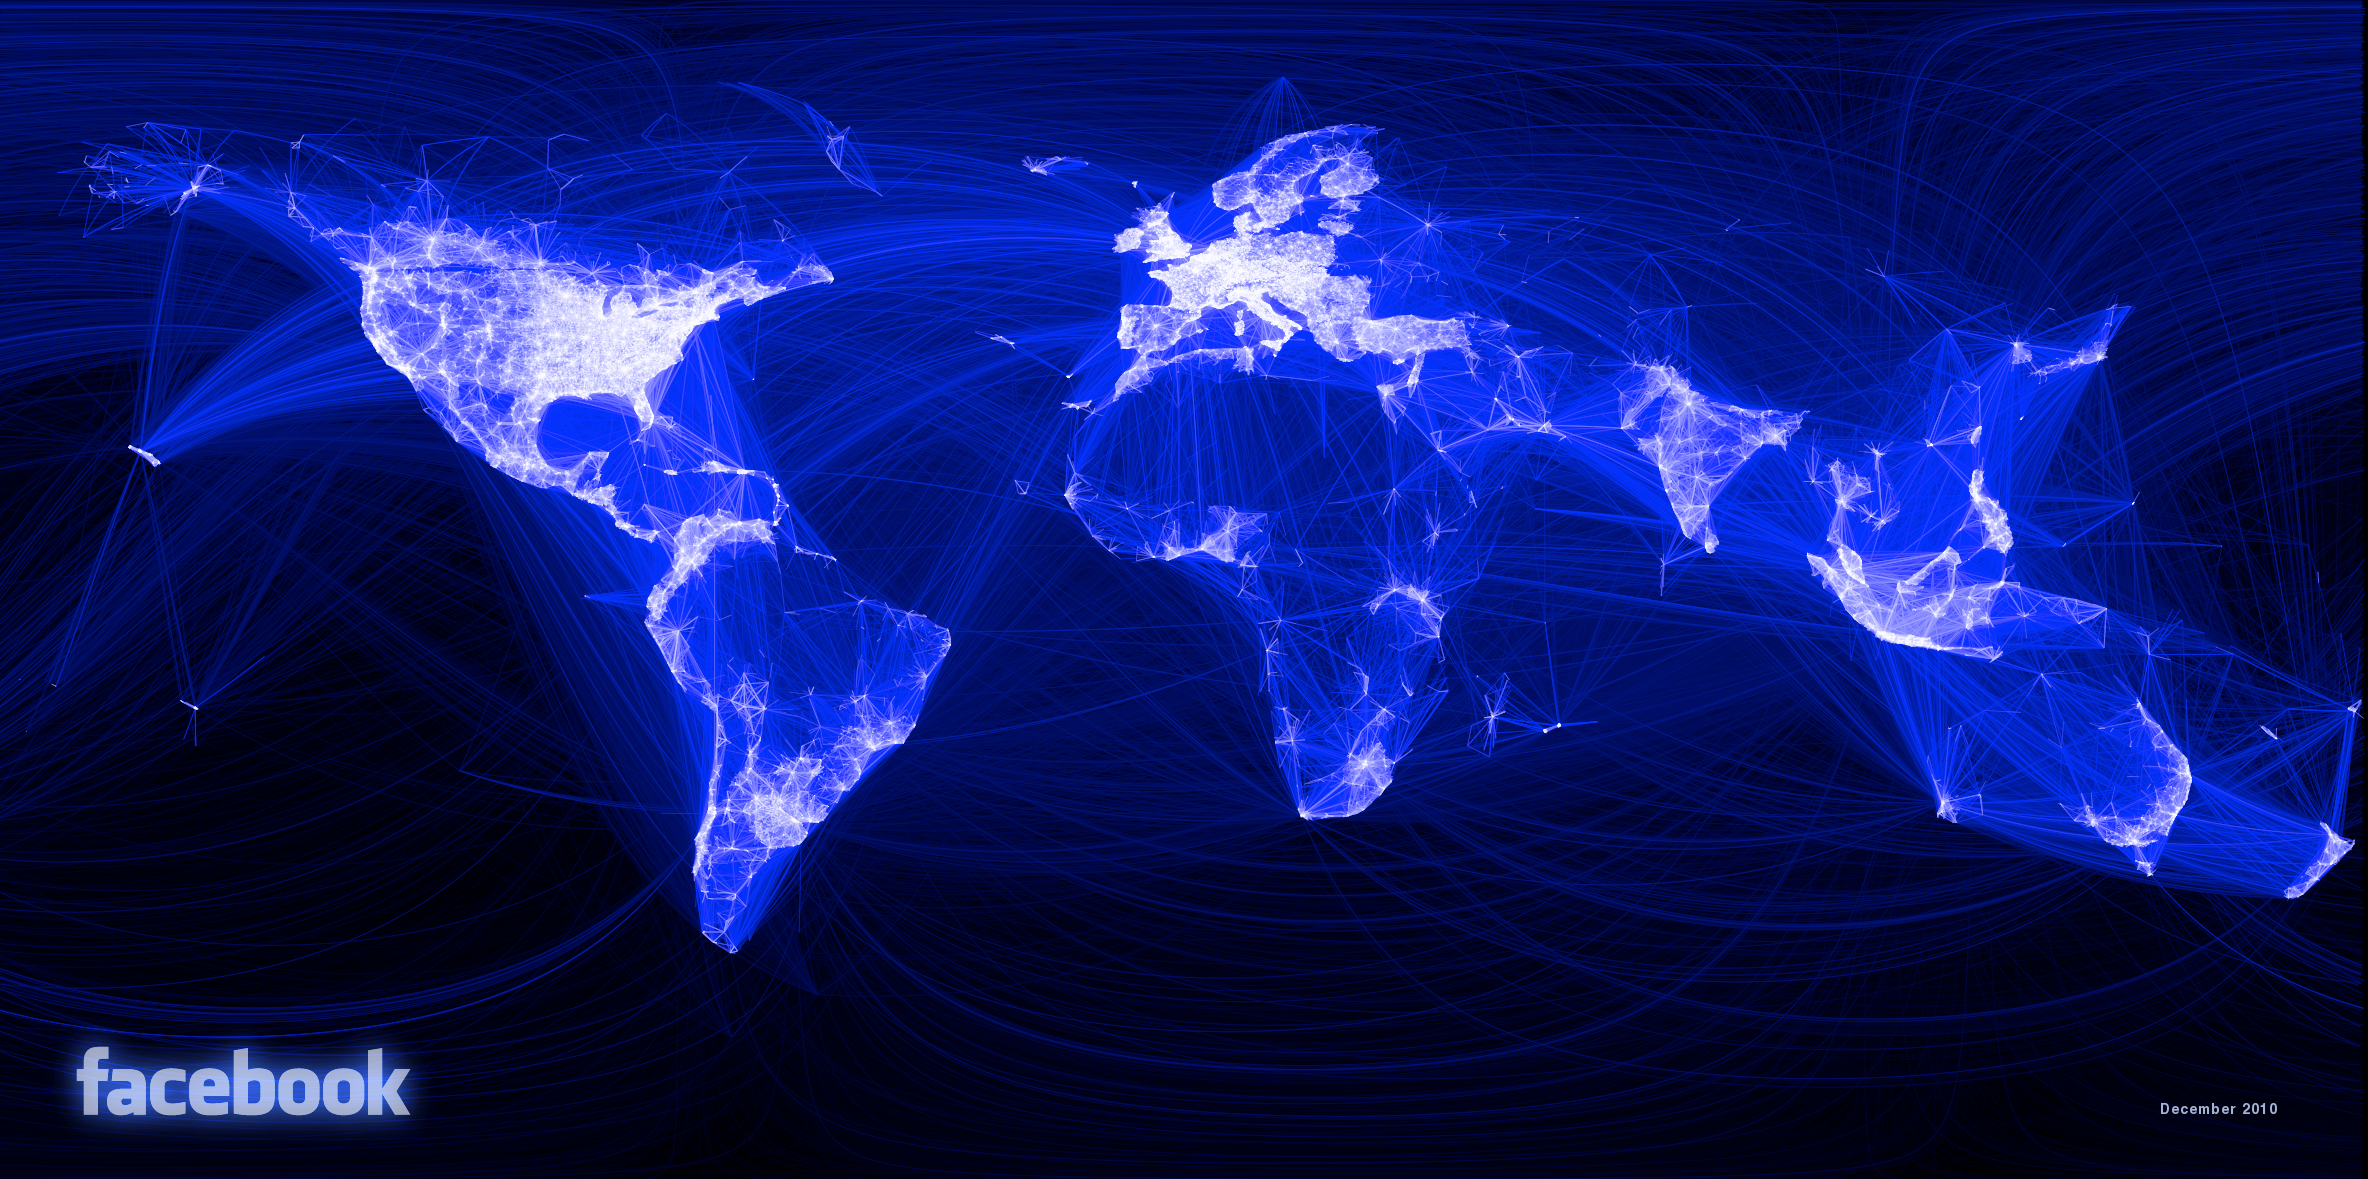
\includegraphics[scale=0.09]{images/facebook}[8]
    \end{center}

\end{frame}
%---

%%% --------------------------
\section{Tips for Visulizations}
%%% --------------------------
\begin{frame}
	\frametitle{Tips for visualizations} 
	\begin{itemize}
		\item Know your audience 
		\item \itshape{ 15 second rule:} \normalfont if your audience won't be able to understand the graphic in 15 seconds, simplify
		\item Layout [9] and font choices
		\item Color choices 
			\begin{itemize}
				\item Available colors in R: 
					\begin{itemize}
						\item \small{\url{http://research.stowers-institute.org/efg/R/Color/Chart/}} \normalfont
					\end{itemize}
				\item Color blindness simulation [11]:
					\begin{itemize}
						\item \url{http://vischeck.com}
						\item \url{http://rsb.info.nih.gov/ij/}
					\end{itemize}
			\end{itemize} 
		\item Add text/labels to figure
	\end{itemize}		


  % \begin{center}
  % 	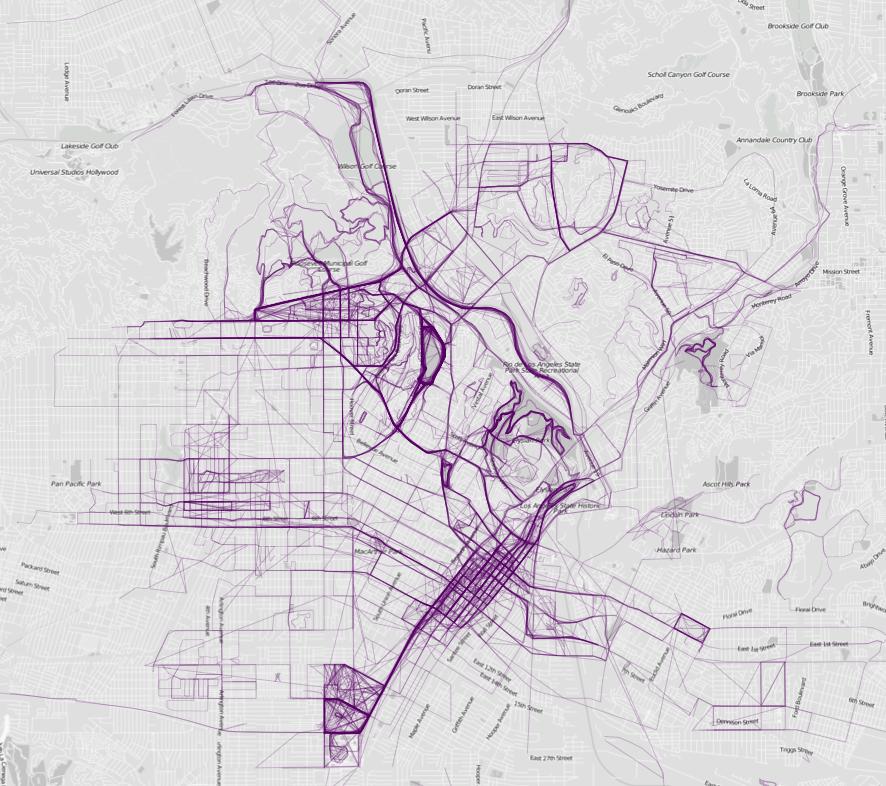
\includegraphics[width=0.4\textwidth]{images/geolocation_ex2}[7]
  % \end{center}

\end{frame}
%---




%%%%%%%%%%%%%%%%%%%%%%%%%%%%%%%%%%%%%
\part{Introduction to R}
%%%%%%%%%%%%%%%%%%%%%%%%%%%%%%%%%%%%%

%%% --------------------------
\section{Installing R and RStudio}
%%% --------------------------
\begin{frame}
  \frametitle{Installing R and RStudio}
  		\vspace{-5pt}
        \begin{enumerate}
           \item[R:] Go to \small \url{http://cran.r-project.org/}, select your operating system and download the latest version: 3.2.3 (Release 2015/12/10).
           \item[RStudio:] Go to \small \url{https://www.rstudio.com/products/rstudio/download/}, select your operating system and download the installer (if available).
        \end{enumerate}
%
		\vspace{-5pt}
       \begin{center}
         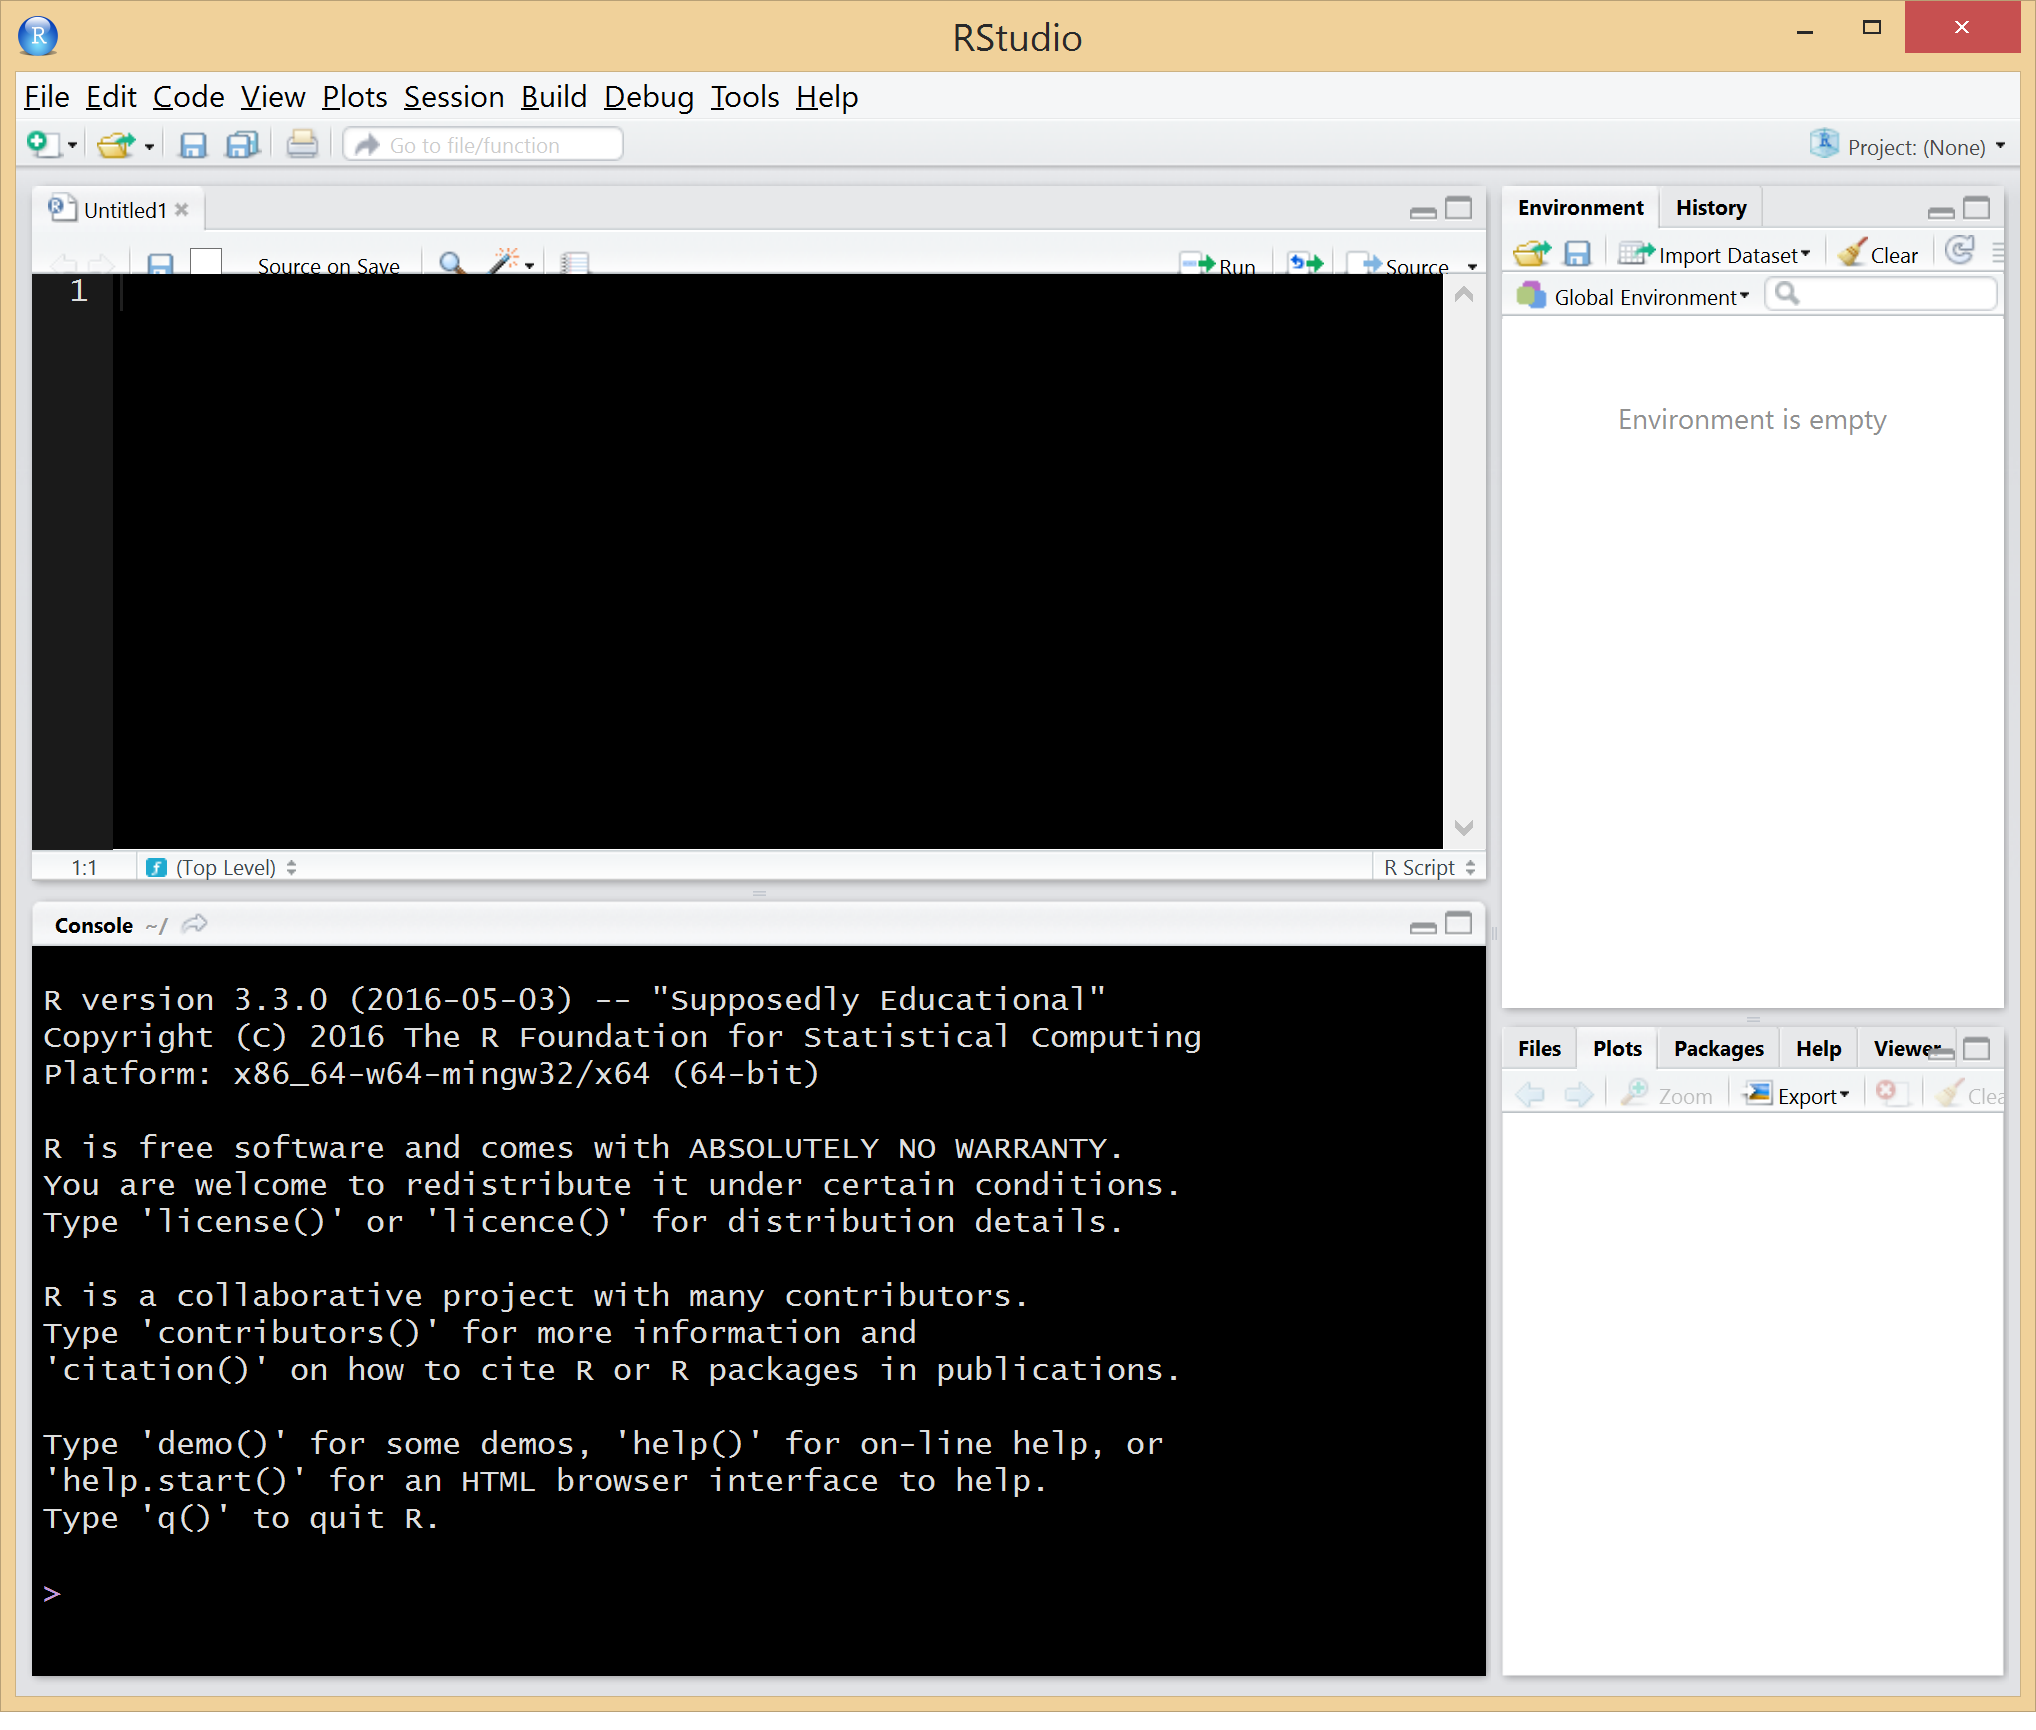
\includegraphics[width=0.5\textwidth]{images/Rwindow.png}
        \end{center}
\end{frame}


%%% --------------------------
\section{Overview of R}
%%% --------------------------
\begin{frame}
	\begin{center}
  		\begin{block}{Overview of R per John Chambers [1]:} 
			"To understand computations in R, two slogans are helpful:
			\begin{itemize}
			        \item Everything that exists is an object.
			        \item Everything that happens is a function call."
			\end{itemize}
		\end{block}
	\end{center} 

% R is flexible: 
% 	\begin{itemize}
% 		\item Objects can be variables, data sets, etc. and can be self-created, downloaded off the web (or elsewhere) and loaded from package(s).
% 		\item Functions (which do something to objects) can also be self-created, downloaded off the web (or elsewhere) and loaded from package(s).
% 		\item A package (1 of 7500+) is a collection of data sets and/or functions unified with a common theme.
% 	\end{itemize}
\end{frame}

%%% --------------------------
\subsection{Creating Objects}
%%% --------------------------
\begin{frame}[allowframebreaks]
	\frametitle{Objects in R}
		\begin{block}{Creating objects in R}
Objects can be created in different ways, via:
			\begin{itemize}
				\item equal sign: \lstinline$ x = 3 $
				\item left arrow: \lstinline$ y <- 2 * x + 1 $
				\item right arrow: \lstinline$ 10 -> z $
			\end{itemize}
		\end{block}

\newpage
	\begin{block}{Examples of Objects}
		\begin{itemize}
			\item[]
			\item Variables, which can be either discrete or continuous:
				\begin{itemize} 
					\item[Discrete:] e.g. number of people at the tutorial
					\item[Continuous:] e.g. how long it took to get to the tutorial
				\end{itemize}
			\item[]
			\item Data frames, which contain data sets with at least one variable:
				\begin{itemize} 
					\item[EX 1:] e.g. data set of commonly performed procedures at CA hospitals (variables include hospital name, procedure type, number of patients who had that procedure, etc.)
					\item[EX 2:] e.g. data set of popular movies (variables include movie name, genre, lead actor/actress, etc.)
				\end{itemize}
		\end{itemize}
	\end{block}

\end{frame}

%%% --------------------------
\subsection{(Very) Brief Overview of Functions}
%%% --------------------------
\begin{frame}[fragile]
	\frametitle{Functions in R}
	\vspace{-15pt}
	\begin{center}
		\begin{block}{Function by example}
			\begin{lstlisting}[ basicstyle=\tiny]
f <- function(x, y=1){
	answer <- x * 2 + y + 1
	return(answer)
}

f(2)        # 6
f(3, 2)     # 9
f(y=3, 2)   # 8
f(y=3, x=3) # 10
			\end{lstlisting}	
		\end{block}

		\vspace{-5pt}
		\begin{block}{Components of a function:}
			\begin{itemize}
				\item Assign function to a variable
				\item Add the 'function' keyword
				\item Specify arguments (if any) that function needs to compute result
				\item Specify any argument defaults
			\end{itemize}
					%%% Assignment, arguments, named, order, unnamed
		\end{block}
	\end{center} 
\end{frame}

%%% --------------------------
\subsection{Comparisons}
%%% --------------------------
\begin{frame}[fragile]
\frametitle{Making Comparisons}
Comparisons return a TRUE or FALSE depending on the condition evaluated:
			\begin{lstlisting}
# Suppose x and y are:
x = 3
y = 5
			\end{lstlisting}
			\begin{lstlisting}[ basicstyle=\footnotesize]
What should the following comparisons return?
x == 3  # is x 3?
x != y  # are x and y different?
x >= y  # is x greater than or equal to y?
(x==3) & (y==4) # is it true that x is 3 and y is 4?
(x==3) | (y==4) # is it true that x is 3 or y is 4?
			\end{lstlisting}	
\end{frame}

%%% --------------------------
\subsection{(More) Notation}
%%% --------------------------
\begin{frame}[fragile, allowframebreaks]
	\frametitle{Notation/Conventions}

	\vspace{10pt}
	\begin{itemize}
		\item[\%$>$\%:] 'pipe operator' which sends objects on the left-hand side to be processed by functions on the right-hand side [15]
			\begin{itemize}
				\item x \%$>$\% f is equivalent to f(x)
			\end{itemize}
		\item[c():] 'concatenation' which combines objects together
			\begin{lstlisting}
x = 3
y = 5
z = c(x, y) 
z
			\end{lstlisting}
			\begin{verbatim}
[1] 3 5
			\end{verbatim}
		\end{itemize}

\newpage
	\begin{itemize}		
		\item[Brackets:] 'subsetting' which says what observation we are (not) interested in
			\begin{lstlisting}
# Example 1:
z = c(3, 5) 
z[2]
			\end{lstlisting}
			\begin{verbatim}
[1] 5
			\end{verbatim}		
			\begin{lstlisting}
# Example 2:
z = c(3, 5) 
z[ z > 3 ]
			\end{lstlisting}
			\begin{verbatim}
[1] 5
			\end{verbatim}						
	\end{itemize}

\end{frame}


\section{Working with Data}

\subsection{Reading Data from File}

%%%%%%%%%%%%%%%%%%%%%%%%%%%%%%%%%%%%%
% --------------------------------------------------- Slide --
\begin{frame}[fragile, allowframebreaks]
 \frametitle{Reading Data from File}

One approach is via \ttfamily read.table(). \normalfont  In the arguments of the function:
  \begin{itemize}
  \item \ttfamily file: \normalfont specifies the (relative) location, file name and file extension
  \item \ttfamily header: \normalfont if TRUE, tells R to include variables names when importing
  \item \ttfamily sep: \normalfont tells R how the entires in the data set are separated
    \begin{itemize}
      \item \ttfamily sep=",": \normalfont when entries are separated by COMMAS
      \item \ttfamily sep="$\backslash t$":\normalfont \hspace{2.5pt} when entries are separated by TAB
      \item \ttfamily sep=" ": \normalfont when entries are separated by SPACE
    \end{itemize}
   \end{itemize}

\newpage   
   	\begin{lstlisting}[ basicstyle=\footnotesize]
filepath = "http://www.ats.ucla.edu/stat/data/test_missing_comma.txt"
### Other valid paths:
# filepath = "C:/Documents/test_missing_comma.txt"
# filepath = "./test_missing_comma.txt"

df <- read.table(
	file = filepath, 
	header = TRUE, 
	sep = ","
	)
	\end{lstlisting}
\normalfont
\normalsize
\end{frame}

%%% --------------------------
\subsection{Working with Data Frames}
%%% --------------------------
\begin{frame}[fragile, allowframebreaks]
	\frametitle{Working with Data Frames}
	To check that a data set has been read-in correctly: 
	\begin{itemize}
		\item View the complete data set by typing the variable name.  (This is not recommended for large data sets.) 
\begin{lstlisting}
df
\end{lstlisting}

{ \small
\begin{verbatim}
    prgtype gender  id ses schtyp level
1   general      0  70   4      1     1
2    vocati      1 121   4     NA     1
3   general      0  86  NA     NA     1
4    vocati      0 141   4      3     1
5  academic      0 172   4      2     1
6  academic      0 113   4      2     1
7   general      0  50   3      2     1
8  academic      0  11   1      2     1
\end{verbatim}
}

\newpage		
		\item View the first 5 lines of the dataset via \ttfamily head(): \normalfont 
\begin{lstlisting}
head(df, 5) 
\end{lstlisting}

\begin{verbatim}
    prgtype gender  id ses schtyp level
1   general      0  70   4      1     1
2    vocati      1 121   4     NA     1
3   general      0  86  NA     NA     1
4    vocati      0 141   4      3     1
5  academic      0 172   4      2     1
\end{verbatim}

\newpage
		\item View the last 7 lines of the dataset via \ttfamily tail(): \normalfont 
\begin{lstlisting}
tail(df, 7)
\end{lstlisting}

\begin{verbatim}
    prgtype gender  id ses schtyp level
2    vocati      1 121   4     NA     1
3   general      0  86  NA     NA     1
4    vocati      0 141   4      3     1
5  academic      0 172   4      2     1
6  academic      0 113   4      2     1
7   general      0  50   3      2     1
8  academic      0  11   1      2     1
\end{verbatim}		

\newpage
		\item Check the variable names via \ttfamily names(): \normalfont 
\begin{lstlisting}
names(df)
\end{lstlisting}

{ \footnotesize
	\begin{verbatim}
[1] "prgtype" "gender"  "id"      "ses"     "schtyp"  "level"
	\end{verbatim}
}	
		\item Check the size of the data set via \ttfamily dim(): \normalfont 
\begin{lstlisting}
dim(df)
\end{lstlisting}

\begin{verbatim}
[1] 8 6
\end{verbatim}	
		\item See the first 6 entries for variable 'gender' via \ttfamily head(): \normalfont 
\begin{lstlisting}
head(df$gender)
\end{lstlisting}

\begin{verbatim}
[1] 0 1 0 0 0 0
\end{verbatim}	

\newpage
	\item Examine how many unique levels a variable has via \ttfamily unique(): \normalfont
\begin{lstlisting}
unique(df$gender)
\end{lstlisting}

\begin{verbatim}
[1] 0 1
\end{verbatim}	
	\item Examine the counts of levels that a variable has via \ttfamily table(): \normalfont
\begin{lstlisting}
table(df$gender, useNA='always')
\end{lstlisting}

\begin{verbatim}
   0    1 <NA> 
   7    1    0 
\end{verbatim}	

\newpage
		\item View entries for a particular variable:
\begin{lstlisting}
## Returns variable as a row/vector:
df$gender # OR
df[, 'gender'] 
## Returns variable as a column: 
df[ 'gender' ] 
\end{lstlisting}		

{\tiny
\begin{verbatim}
[1] 0 1 0 0 0 0 # OR

  gender
1      0
2      1
3      0
4      0
5      0
6      0
7      0
8      0
\end{verbatim}	
}

\newpage	
		\item View entries for a few variables:
\begin{lstlisting}
head( df[, c('gender', 'ses') ], 3) 
\end{lstlisting}		

\begin{verbatim}
  gender ses
1      0   4
2      1   4
3      0  NA
\end{verbatim}

\newpage
		\item Verify ranges and check for missing data via \ttfamily summary(): \normalfont 
\begin{lstlisting}
summary(df)
\end{lstlisting}

{ \tiny
	\begin{verbatim}
      prgtype      gender            id             ses            schtyp      level  
    vocati:2   Min.   :0.000   Min.   : 11.0   Min.   :1.000   Min.   :1   Min.   :1  
   general:3   1st Qu.:0.000   1st Qu.: 65.0   1st Qu.:3.500   1st Qu.:2   1st Qu.:1  
  academic:3   Median :0.000   Median : 99.5   Median :4.000   Median :2   Median :1  
               Mean   :0.125   Mean   : 95.5   Mean   :3.429   Mean   :2   Mean   :1  
               3rd Qu.:0.000   3rd Qu.:126.0   3rd Qu.:4.000   3rd Qu.:2   3rd Qu.:1  
               Max.   :1.000   Max.   :172.0   Max.   :4.000   Max.   :3   Max.   :1  
                                               NA's   :1       NA's   :2              
	\end{verbatim}	
}
	\end{itemize}
\end{frame}


%%% --------------------------
\section{Adding Functionality to Base R}
%%% --------------------------

\begin{frame}[fragile]
	\frametitle{Adding Functionality to Base R}

	\begin{itemize}
		\item Base R is what you download off CRAN \url{www.cran.r-project.org} 
		\item Available packages are listed here: \url{https://cran.r-project.org/web/packages/}
		\item Install an R package(s) via \ttfamily install.packages(): \normalfont 
   	\begin{lstlisting}[ basicstyle=\small]
install.packages("lattice")
install.packages("ggplot2")
# OR
install.packages( c("lattice", "ggplot2") )

	\end{lstlisting}
	\end{itemize} 	
\end{frame}



%%%%%%%%%%%%%%%%%%%%%%%%%%%%%%%%%%%%%

	
% ------------------------------------------------------------
% ------------------------------------------------------------

\section[Summary Plots]{Summary Plots}

\subsection{Scatterplot}
%%%%% New frame
\begin{frame}[allowframebreaks, fragile]
\frametitle{Scatterplots}

To get a quick peak into the numerical variables in the data \ttfamily scatterplot.matrix(): \normalfont
  		\begin{lstlisting}
library(car)		
data(quakes)
scatterplot.matrix(quakes[, 1:4])
		\end{lstlisting}

        \begin{center}
         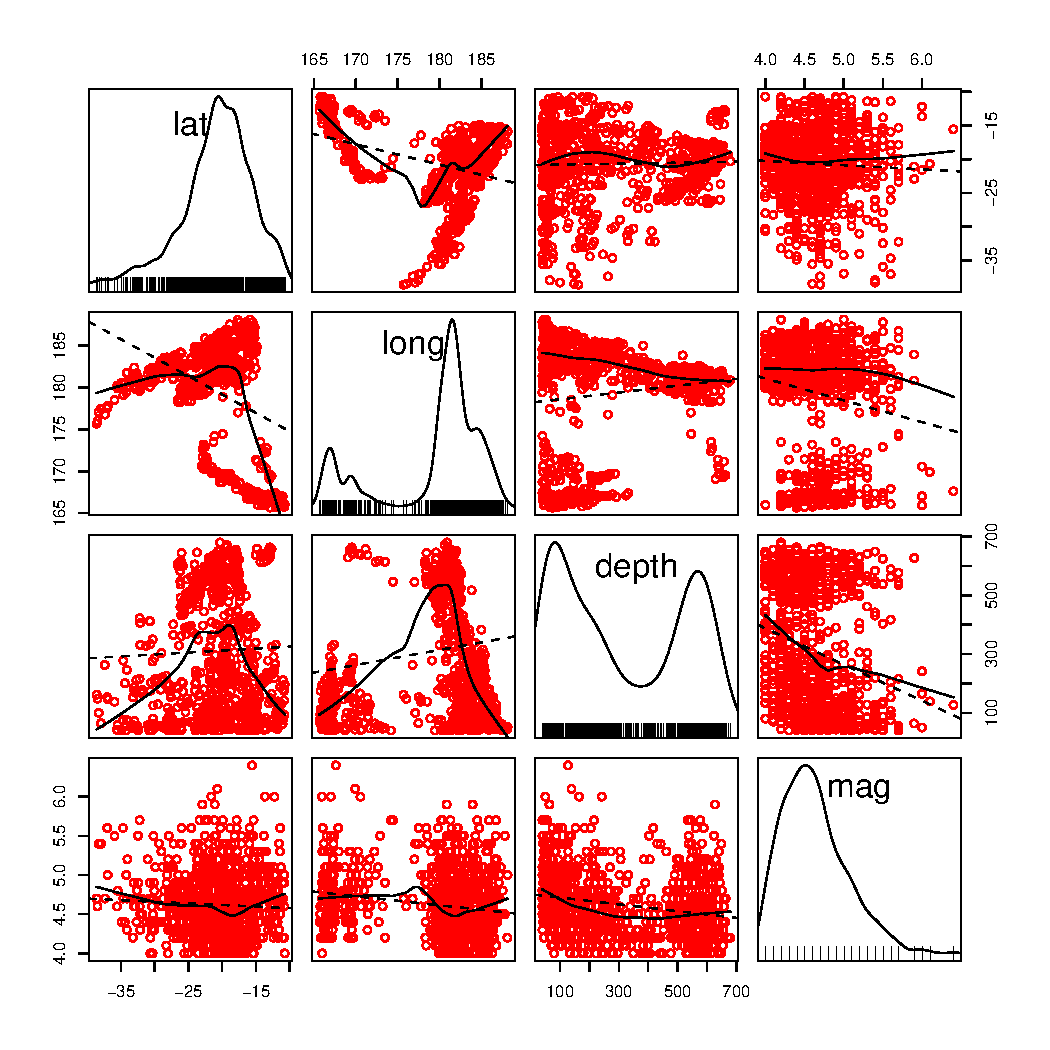
\includegraphics[width=0.63\textwidth]{images/scatterPlot.pdf}
        \end{center}
\end{frame}


%%%%% New frame
\subsection{Histogram}
\begin{frame}[allowframebreaks, fragile]
\frametitle{'Nicer' Histogram}

To compare the frequencies of two variables side-by-side, use \ttfamily beanplot(): \normalfont

	\begin{lstlisting}
library(datasets)
library(beanplot)
data(ToothGrowth)
beanplot(len ~ supp, data=ToothGrowth, col=list(grey(0.5),c(grey(0.8),"white")), border = NA, overallline = "median", ll=0.01, side="both")
legend("bottomleft",fill=c(grey(0.5),grey(0.8)), legend=c("Orange Juice","Ascorbic Acid"))
	\end{lstlisting}
	
        \begin{center}
	         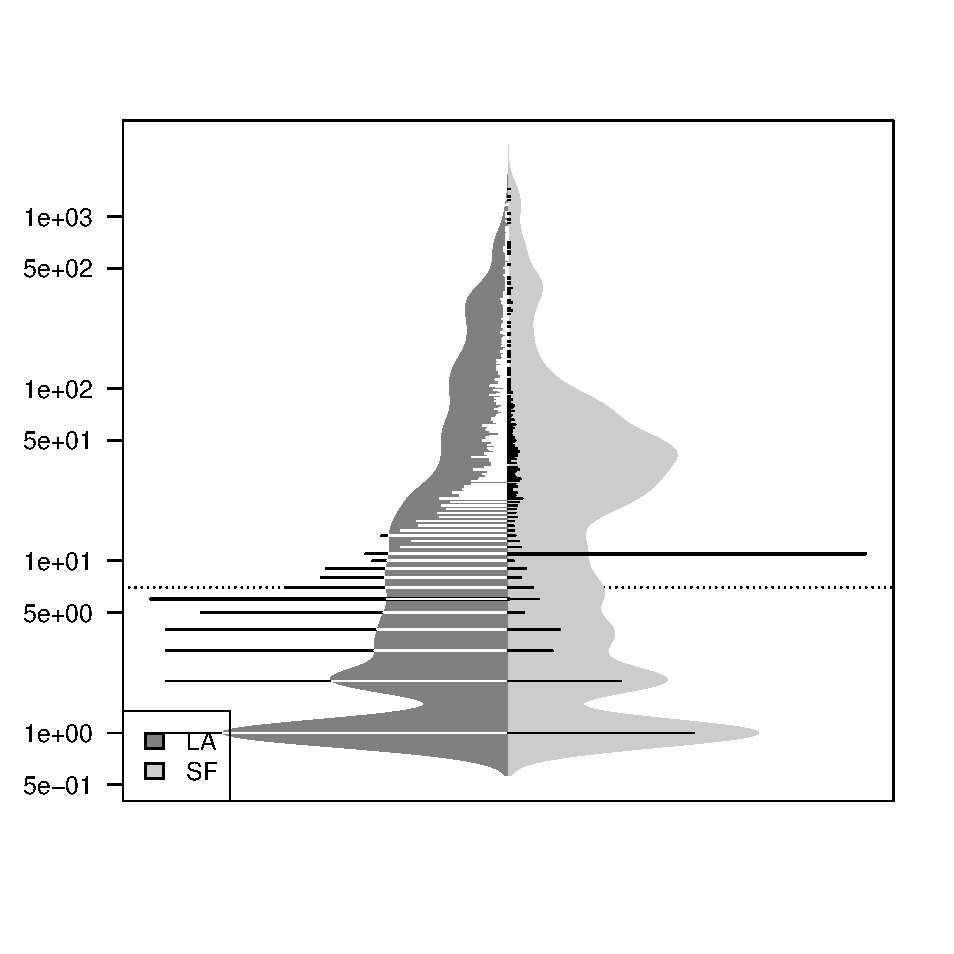
\includegraphics[width=0.65\textwidth]{images/beanplot.pdf}
        \end{center}
\end{frame}

%%% NOT WORK...
%
%library(lattice)
%split.screen(c(1,2))        # split display into two screens
%split.screen(c(2,1),2)      # split bottom half in two
%screen(1)                   # prepare screen 1 for output
%qqplot(ToothGrowth$len~ToothGrowth$supp)
%screen(4)                   # prepare screen 4 for output
% # boxplot(ToothGrowth$len~ToothGrowth$supp)
% beanplot(ToothGrowth$len~ToothGrowth$supp, col=list(grey(0.5),c(grey(0.8),"white")), border = NA, overallline = "median", ll=0.01, side="both")
%screen(1, FALSE)            # return to screen 1, but do not clear
%close.screen(all = TRUE)    # exit split-screen mode


%%%%%%%%%%%%%%%%%%%%%%%%%%%%%%%%%%%%%

% ------------------------------------------------------------
% ------------------------------------------------------------

% Exercise: compare distributions of Iris data
% ID outlier in dataset

\subsection{Exercise I}
\begin{frame}
	\frametitle{Exercise I}
	Compare the distributions of the sepal widths for the three species of irises (using the \ttfamily iris \normalfont data set).
\end{frame}
		% pie chart, histogram
	% http://www.r-bloggers.com/time-series-plots-in-r/
% http://www.fromthebottomoftheheap.net/2013/10/23/time-series-plots-with-lattice-and-ggplot/


% ------------------------------------------------------------
% ------------------------------------------------------------

%%%%%%%%%%%%%%%%%%%%%%%%%%%%%%%%%%%%%

% Section: Plots of TS in R 

\section[Time Series Plots]{Time Series Plots}
%%%%%%%%%%%%%%%%%%%%%%%%%%%%%%%%%%%%%

\subsection{Univariate Time Series Plots}
%%%%%%%%%%%%%%%%%%%%%%%%%%%%%%%%%%%%%%

\begin{frame}[fragile, allowframebreaks]
\frametitle{Univariate Time Series Plots}

One way to plot one variable at a time (over time), is via \ttfamily plot(): \normalfont 
		\begin{lstlisting}
### Step 0: Load any required packages:
library(dplyr)

### Step 1: Get yearly counts across hospitals and procedures
df_summary <- df_clean %>%
  group_by(Year) %>%
  summarise(Total.for.Year = sum(Volume, na.rm=TRUE))
  \end{lstlisting}

\newpage
  \begin{lstlisting}
### Step 3: Visualize
plot(
  x=df_summary$Year,
  y=df_summary$Total.for.Year,
  xlab="Year",
  ylab="Volume",
  type="b",
  main="Yearly Volume for 6 procedures in CA"
  )
		\end{lstlisting}
What are some limitations of the data set (and hence plot)?

\newpage
      \begin{center}
        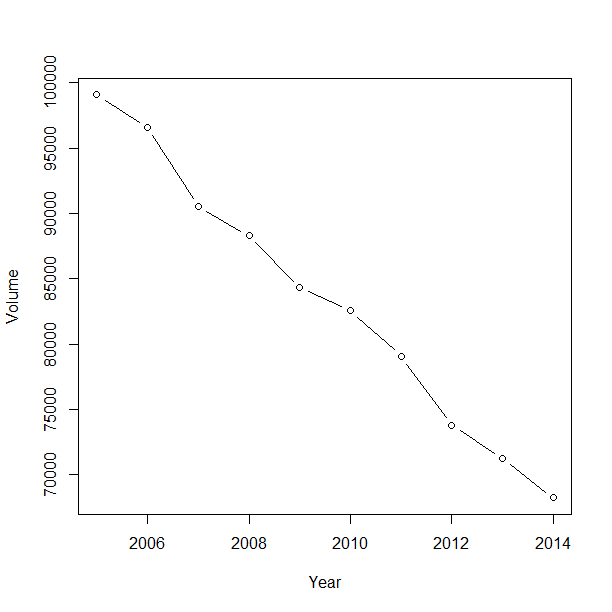
\includegraphics[width=0.6\textwidth]{images/univar_ts.png}
       \end{center}

\end{frame}

%%%%%%% New frame
%\begin{frame}[allowframebreaks, fragile]
% \frametitle{Customizing the plot}

%To plot more than variables one at a time, use \ttfamily xyplot(): \normalfont
%		\begin{lstlisting}
%# After processing data as in Approach 1
%# load both libraries:
%library(lattice)
%library(zoo)
%data(EuStockMarkets)
%z<-EuStockMarkets
%xyplot(z, screen = c(1,1,1,1), col = 1:4, strip = FALSE)
%legend(1992, 5000, colnames(z), lty = 1, col = 1:4)
%		\end{lstlisting}

%       \begin{center}
%         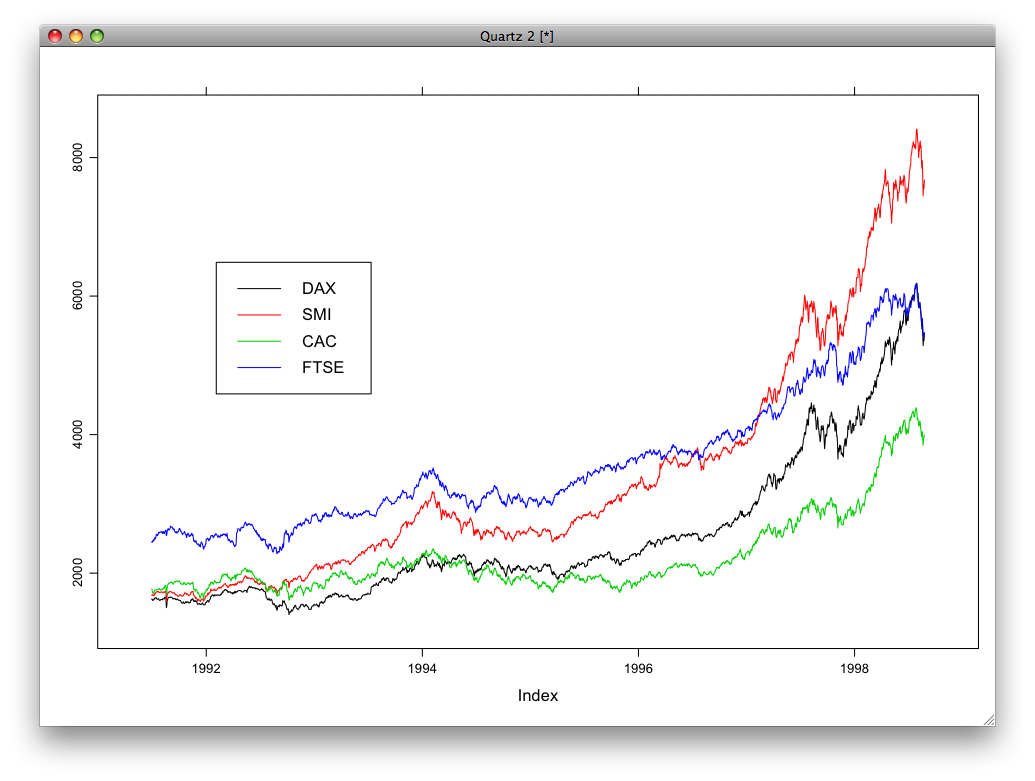
\includegraphics[width=0.85\textwidth]{images/stockPlot2}
%        \end{center}
%\end{frame}

%%%%%%%%%%%%%%%%%%%%%%%%%%%%%%%%%%%%%

\subsection{Multivariate Time Series Plots}

%%%%%%%%%%%%%%%%%%%%%%%%%%%%%%%%%%%%%

\begin{frame}[allowframebreaks, fragile]
 \frametitle{Multivariate Time Series Plots: Approach 1}

To plot more than one variable at a time, over time, you can ttfamily \use xyplot()\normalfont [5]:
%\begin{itemize}
%	\item For documentation, go to: www.jstatsoft.org/v25/c01/paper 
%	\item Go to: http://www.biostat.jhsph.edu/$\sim$rpeng/RR/mvtsplot/
%	\item Copy the relevant R Code and paste it into the R Console. Press ENTER.
%	\item Plot your data
% \end{itemize}
		\begin{lstlisting}
### Step 0: Load any required packages
library(dplyr)
library(lattice)

### Step 1: Get data for one procedure
df_LA_CABG <- df %>%
  filter( 
    (County == "Los Angeles") & 
    (Procedure == "CABG") & 
    (Volume > 0) 
    )
    \end{lstlisting}

\newpage    
    \begin{lstlisting}
### Step 2: Visualize    
xyplot( Volume ~ Year | Hospital.Name, 
  data=df_LA_CABG,
  par.strip.text=list(cex=0.5),
  type="b",
  main="LA Coronary artery bypass grafting (CABG)"
  )
		\end{lstlisting}

\newpage
      %\vspace{-30pt} 
      \begin{center}
        %\hspace{-25pt}
         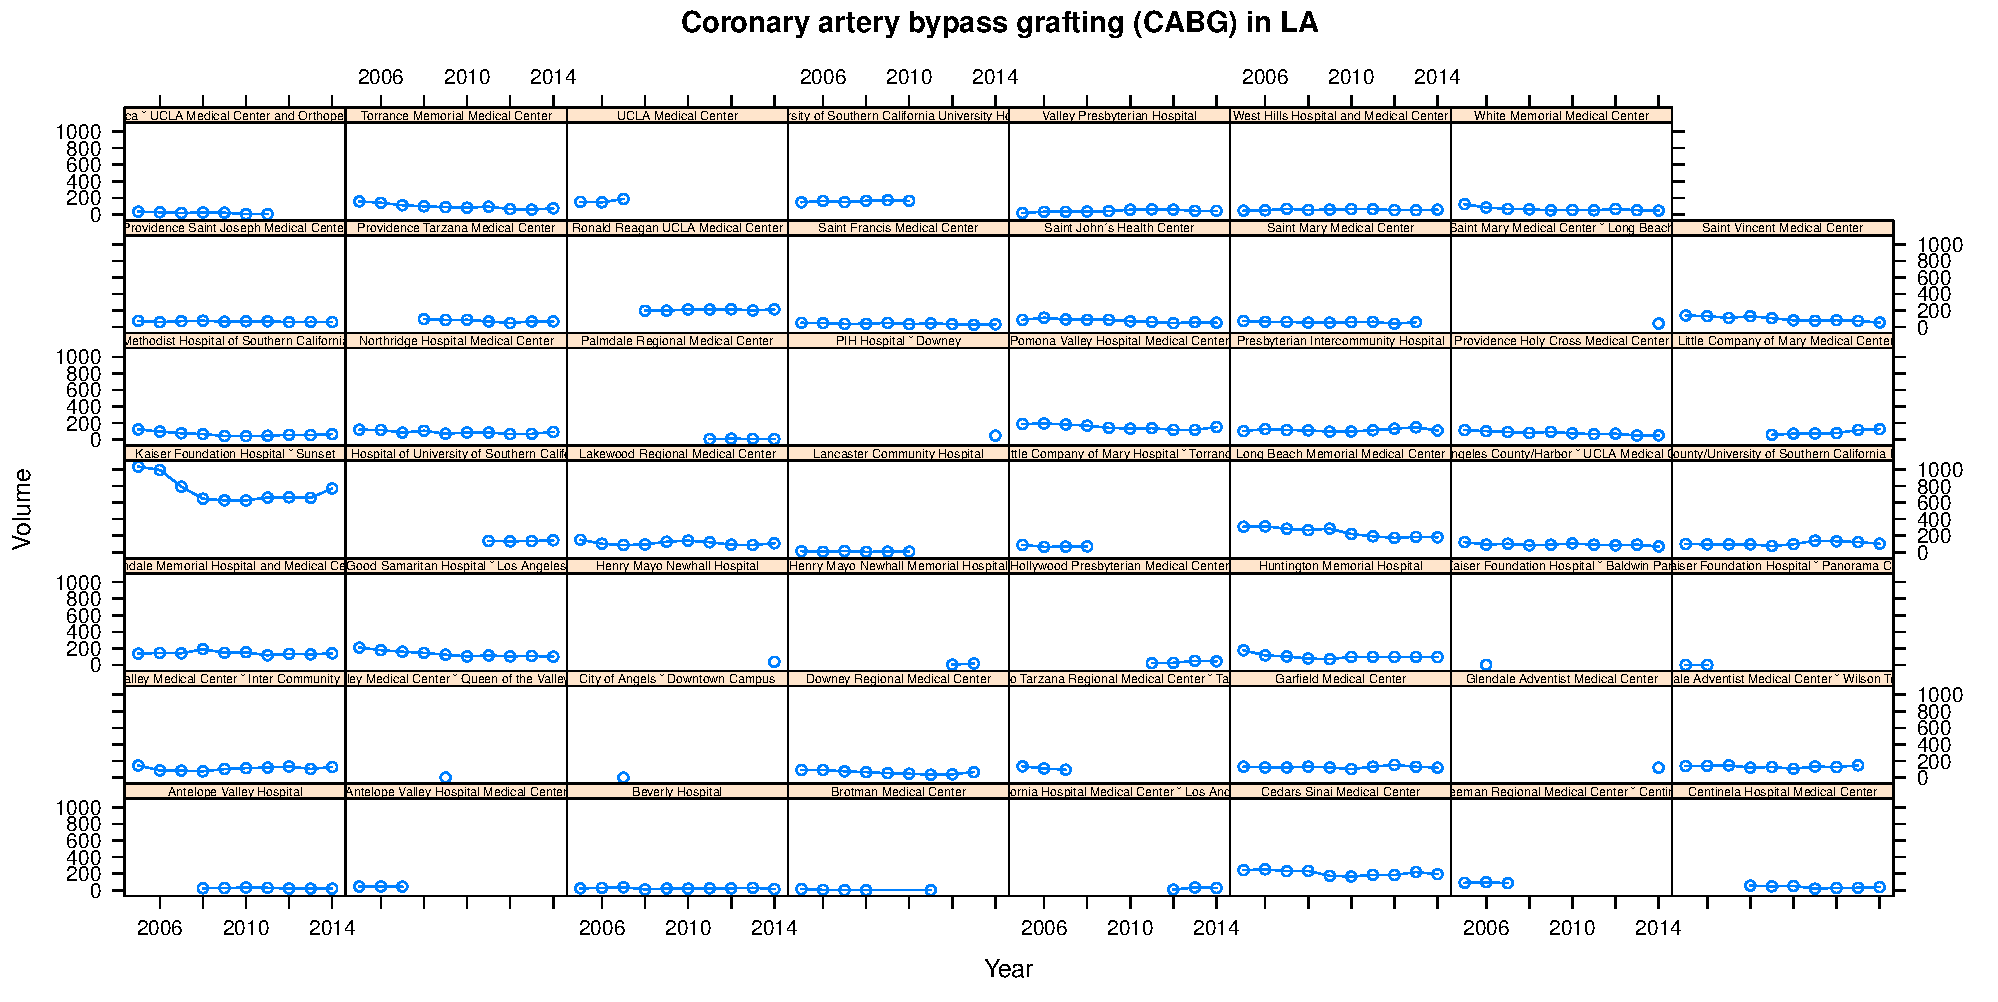
\includegraphics[width=1.05\textwidth]{images/timeseries_LA_CABG}
      \end{center}
\end{frame}

%---
\begin{frame}[fragile, allowframebreaks]
 \frametitle{Multivariate Time Series Plots: Approach 2}

Another way to plot more than one variable at a time, is via \ttfamily ggplot()\normalfont :

    \begin{lstlisting}
### Step 0: Load any required packages:
library(dplyr)
library(ggplot2)

### Step 1: Get data for one hospital:
df_Cedars <- df_clean %>%
  filter( Hospital.Name == 'Cedars Sinai Medical Center')
   \end{lstlisting}

\newpage
    \begin{lstlisting}
### Step 2: Visualize
ggplot( data = df_Cedars ) + 
  geom_line( aes(
    x = Year, 
    y = Volume, 
    linetype = Procedure) ) +
  scale_x_continuous( breaks=seq(
    from=2005, 
    to=2014, 
    by=3) ) +
  theme_classic() +
  ggtitle( "Volume of Procedures for Cedars Sinai Medical Center" )
   \end{lstlisting}

\newpage
       \begin{center}
         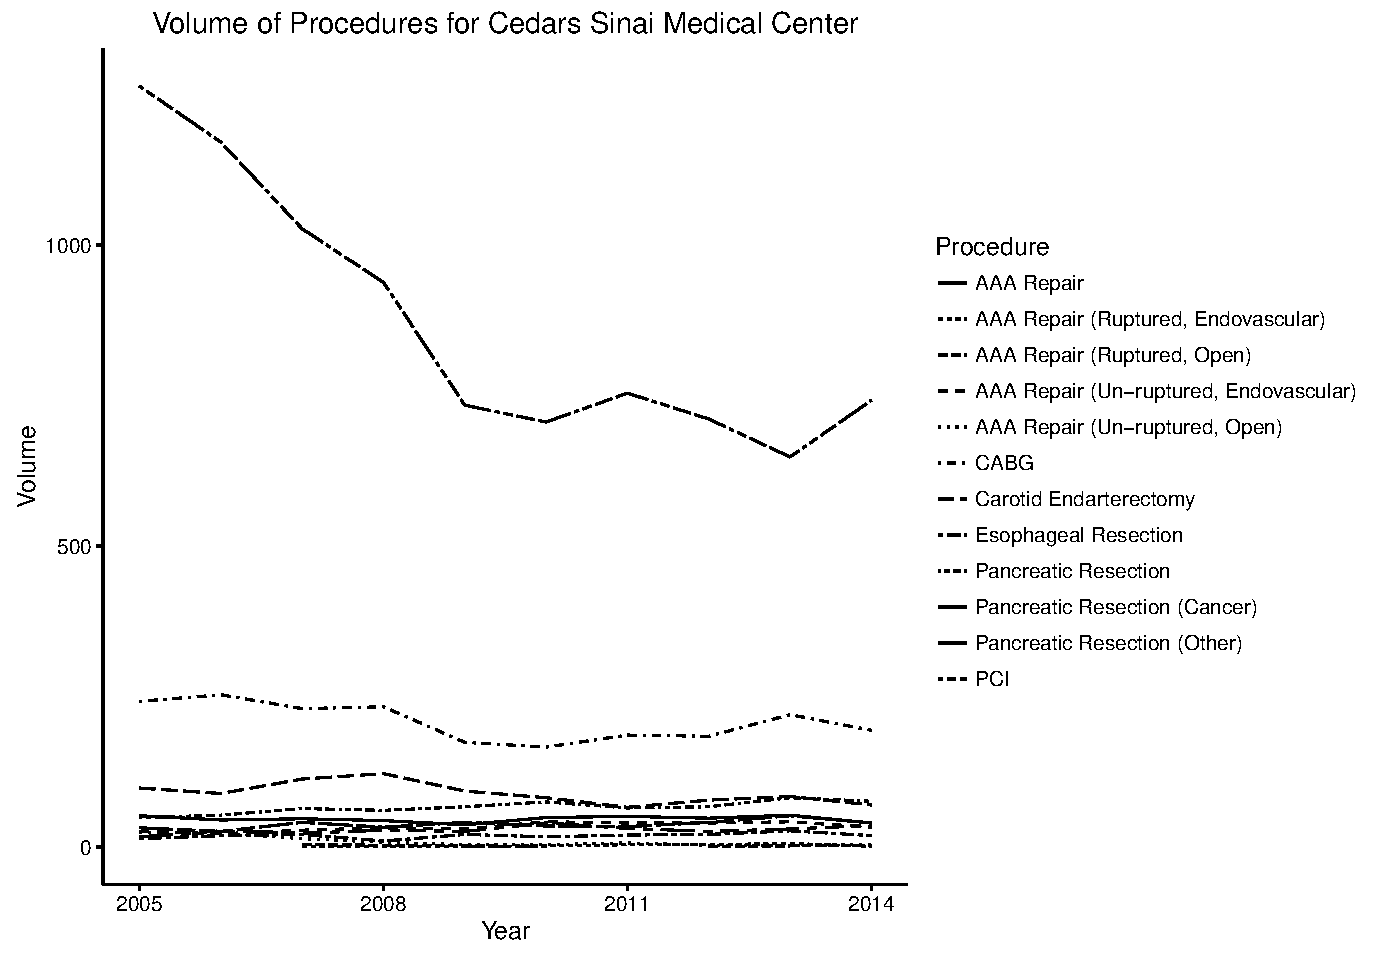
\includegraphics[width=0.9\textwidth]{images/timeseries_Cedars}
        \end{center}
\end{frame}

% % ------------------------------------------------------------
% % ------------------------------------------------------------
\subsection{Exercise II}
\begin{frame}[fragile]
	\frametitle{Exercise II}
	In the healthcare data set, recently what seems to be the most popular procedure in CA?\\
  \vspace{10pt}
  \noindent Hints: \small
    \begin{itemize}
      \item Should we aggregate the data?  If so, to what level?
      \item What's one way to examine trends in the data?
    \end{itemize}

    \normalsize
\end{frame}

		% mtvsplot, plot, xyplot
		% changing plotting options
	
% ------------------------------------------------------------
% ------------------------------------------------------------

\section[Geographical Plots]{Geographical Plots}
%%%%%%%%%%%%%%%%%%%%%%%%%%%%%%%%%%%%%
\subsection{Plots using Maps}
%%%%%%%%%%%%%%%%%%%%%%%%%%%%%%%%%%%%%

\begin{frame}[fragile, allowframebreaks]
\frametitle{Geographic Maps (v0.1)}

To overlay a map to a plot containing latitude and longitude, load the package \ttfamily maps: \normalfont 

\begin{lstlisting}[ basicstyle=\footnotesize]
library(maps)
plot(
 x = df_clean$Longitude, 
 y = df_clean$Latitude,
 xlab = "Longitude",
 ylab = "Latitude",
 pch = 16,
 col = rgb(176/256, 196/256, 222/256, alpha=0.5)
)
map("state", "california", add=TRUE)
\end{lstlisting}

\newpage
	\begin{center}
		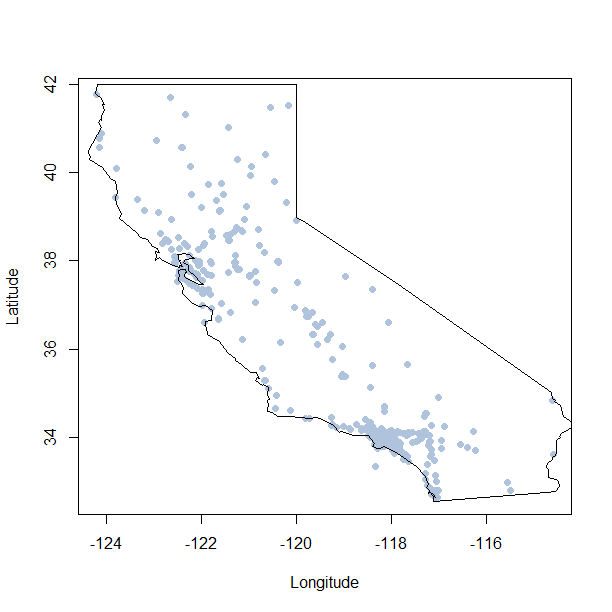
\includegraphics[scale=0.25]{images/geoplot_v0.png}
	\end{center}
What are some limitations of the plot?
\end{frame}

%___________
\begin{frame}[fragile, allowframebreaks]
\frametitle{Geographic Maps (v0.2)}

To include information on volume of procedure, use \ttfamily cex\normalfont argument of the \ttfamily plot() \normalfont function:

\begin{lstlisting}[ basicstyle=\footnotesize]
### Step 1: Aggregate data to be at hospital level:
df_hosp <- data_clean %>%
  group_by( Latitude, Longitude ) %>%
  summarise( Total.for.Hospital = sum(Volume, na.rm=TRUE) )
	
### Step 2: Recode 'Volume' to have 2 categories only: high ( >100 cases ) and low ( <= 100 cases ):
df_hosp$volume_ind <- ifelse( 
 test = df_hosp$Total.for.Hospital > 100, 
 yes = 2, 
 no = 1 )
\end{lstlisting}

\newpage
\begin{lstlisting}
### Step 3: Plot
plot(
 x = df_hosp$Longitude, 
 y = df_hosp$Latitude, 
 pch = 19, 
 cex = df_hosp$volume_ind, 
 col = df_hosp$volume_ind, 
 xlab = "Longitude", 
 ylab = "Latitude",
 main="Indicator of overall volume between 2005-2014"
)
map("state", "california", add=TRUE)
\end{lstlisting}

\begin{lstlisting}
### Step 4: Add legend
legend("topright", 
 pch = 19, 
 pt.cex = 1:2,
 col = 1:2, 
 c("Vol <= 100", "Vol > 100") 
)
\end{lstlisting}

\newpage
       \begin{center}
		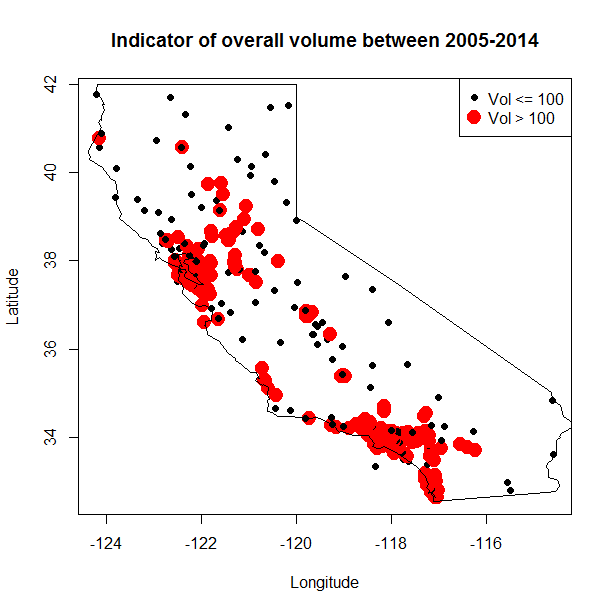
\includegraphics[scale=0.25]{images/geoplot_v1.png}
	\end{center}
What are some limitations of the plot? (Exercise.)
\end{frame}

%---
\begin{frame}[fragile, allowframebreaks]
\frametitle{Geographic Maps (v0.3)}

Another way to visualize geographical information is via shapefiles. Please download shapefiles for California for 2014 from \url{https://www.census.gov/geo/maps-data/data/cbf/cbf_tracts.html} and unzip the folder.

\begin{lstlisting}
### Step 1: Load in required packages
library(sp)
library(rgdal)
\end{lstlisting}

\newpage
\begin{lstlisting}
### Step 2: Read in shapefile and add latitude and longitude coordinates to it:
tracts = spTransform(
	readOGR(
		file.path("cb_2014_06_tract_500k"), 
		layer = "cb_2014_06_tract_500k"
		), 
	CRS("+proj=longlat +datum=WGS84")
	) 

### Step 3: Visualize
plot(tracts)
\end{lstlisting}

\newpage
       \begin{center}
		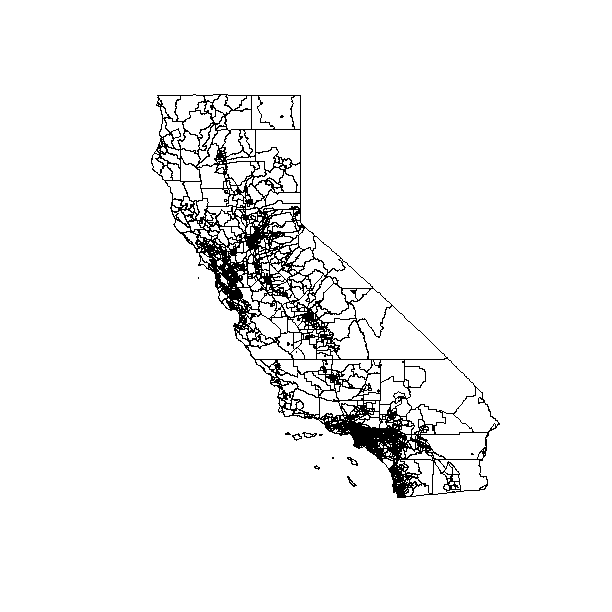
\includegraphics[scale=0.25]{images/shapefile_v0.png}
		\caption{Plot of the shapefile tracts.}
	\end{center}

\newpage
Now let's add the locations of hospitals to the map [12]:

\begin{lstlisting}
### Step 1: Load required packages
library("rgdal") 
library("maptools")
library("ggplot2")
library("plyr")

### Step 2: Preprocess data ahead of plotting
tracts@data$id = rownames(tracts@data)
tracts.points = fortify(tracts, region="id")
tracts.df = join(
 tracts.points, 
 tracts@data, 
 by="id"
 )
\end{lstlisting}

\newpage
\begin{lstlisting}
### Step 3: Visualize
ggplot() +
  geom_polygon(data = tracts.df,
               aes(x = long, y = lat, group = group),
               fill = grey(0.6), 
               color = grey(0.6), 
               alpha = 0.5
               ) + 
  geom_point(data = df_hosp,
             aes(x = Longitude, y = Latitude),
             color = "blue4", 
             alpha = 0.5, 
             shape = 3,
             size = 2 )
\end{lstlisting}

\newpage
       \begin{center}
		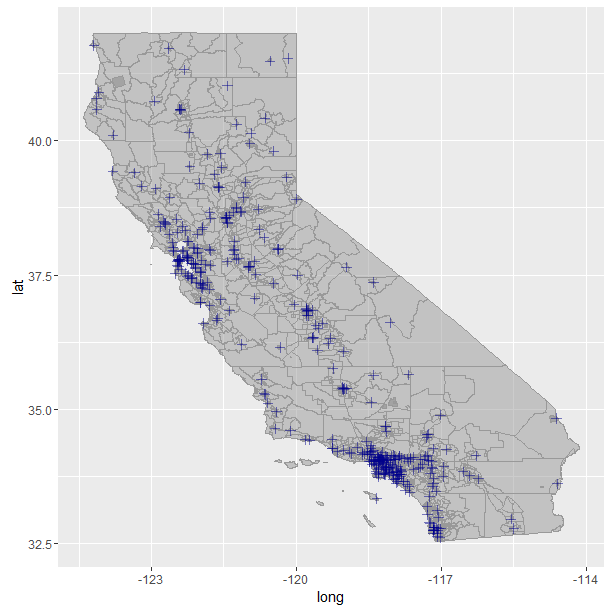
\includegraphics[scale=0.3]{images/shapefile_v1.png}
	\end{center}

\end{frame}

%%%%%%%%%%%%%%%%%%%%%%%%%%%%%%%%%%%%%
\subsection{Interactive Geographical Plots}
%%%%%%%%%%%%%%%%%%%%%%%%%%%%%%%%%%%%%
\subsubsection{Geographical Plots via 'ggvis'}
\begin{frame}[fragile, allowframebreaks]
	\frametitle{Geographical Plots via 'ggvis'}
One way to make high resolution and interactive images is via 'ggvis' [13]:

\begin{lstlisting}[ basicstyle=\footnotesize]
# Please note, it may take some time to load as the shapefile is high resolution:
library(ggvis)
tracts.points %>%
  ggvis(~long, ~lat) %>%
  group_by(group, id) %>%
  layer_paths(strokeOpacity:=0.5, stroke:=grey(0.5)) %>%
  layer_points(data=df_hosp, x=~Longitude, y=~Latitude, size:=8) %>%
  hide_legend("fill") %>%
  set_options(width=400, height=400, keep_aspect=TRUE)
\end{lstlisting}

\newpage
       \begin{center}
		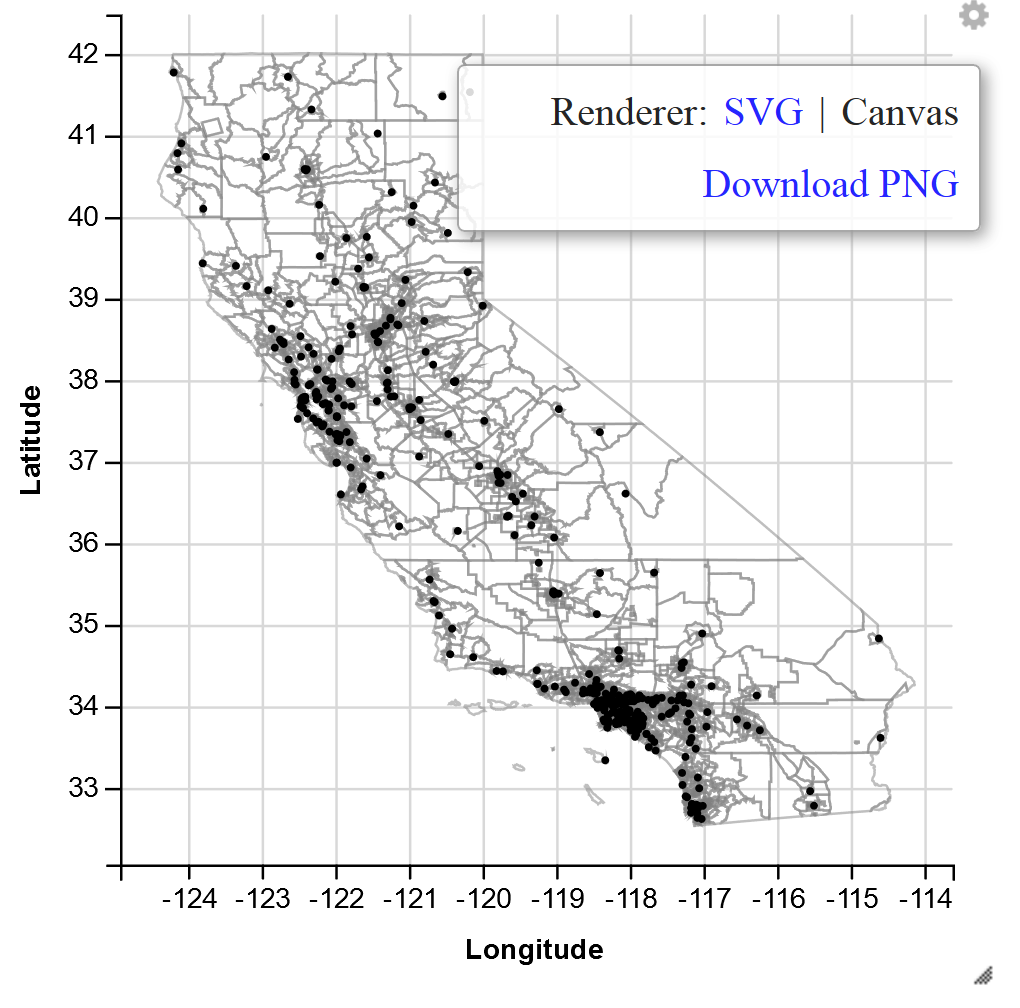
\includegraphics[scale=0.6]{images/shapefile_v2.png}
	\end{center}

\newpage
Now we can add (basic) interactivity by resizing the hospital locations:

\begin{lstlisting}[ basicstyle=\tiny]
library(ggvis)
tracts.points %>%
  ggvis(~long, ~lat) %>%
  group_by(group, id) %>%
  layer_paths(
    strokeOpacity:=0.5, 
    stroke:=grey(0.5)) %>%
  layer_points(
    data=df_hosp, 
    x=~Longitude, 
    y=~Latitude, 
    size:=input_slider(8, 100, value = 12, label='Point size')) %>%
  hide_legend("fill") %>%
  set_options(width=400, 
    height=400, 
    keep_aspect=TRUE)
\end{lstlisting}

\newpage
  \begin{center}
    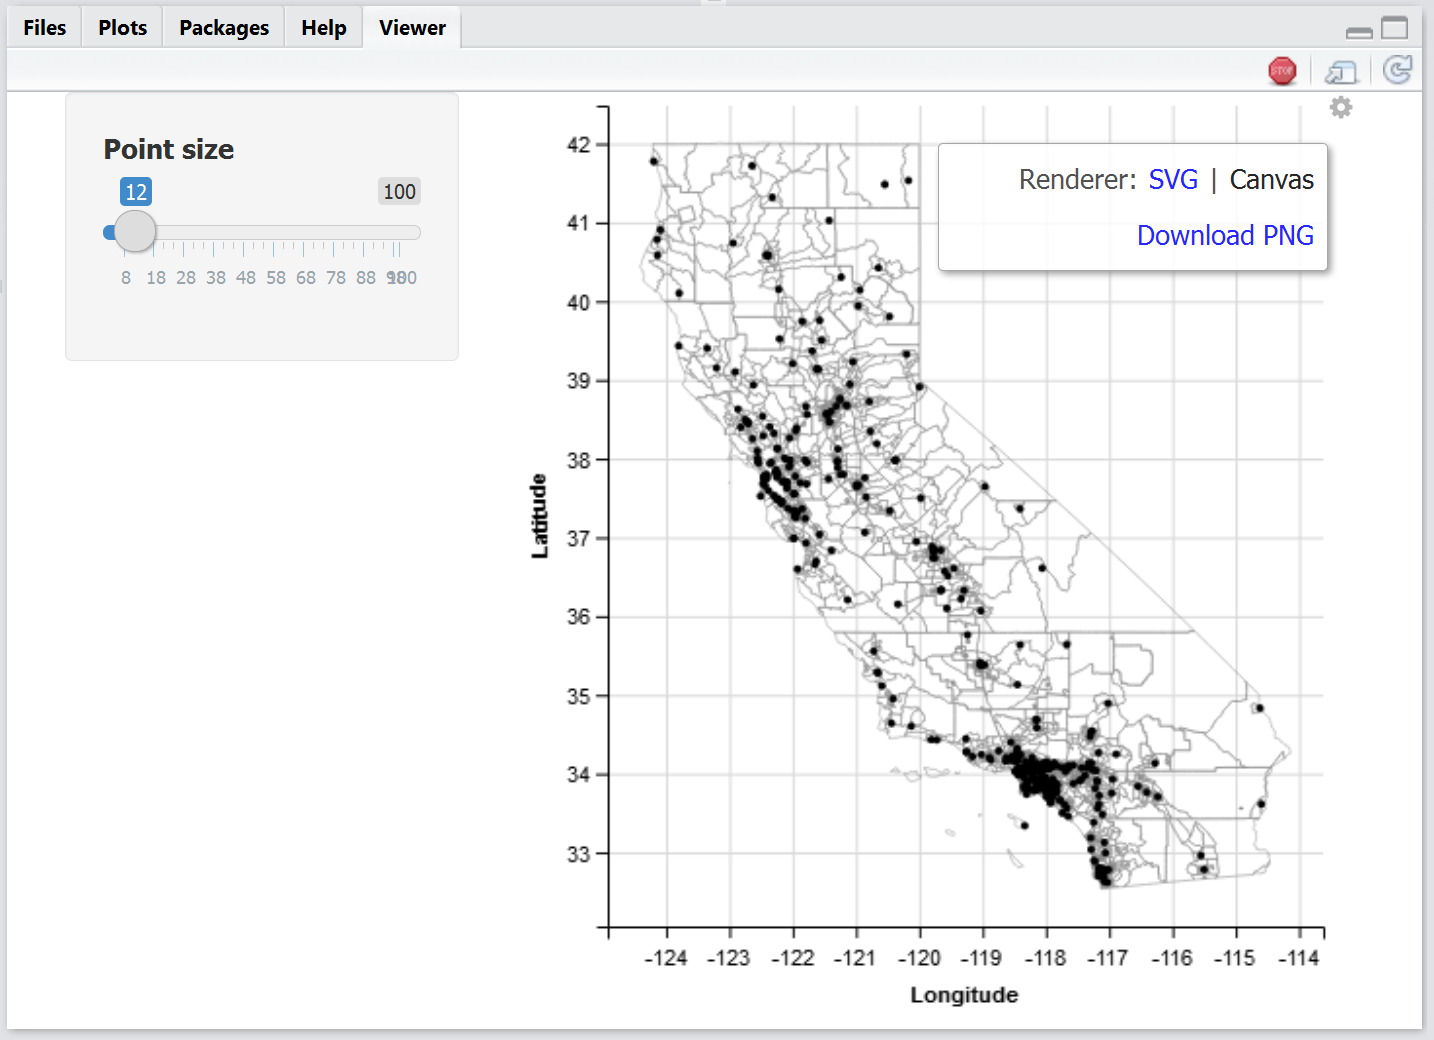
\includegraphics[scale=0.55]{images/shapefile_v3-4-1.png}
  \end{center}

\newpage
  \begin{center}
    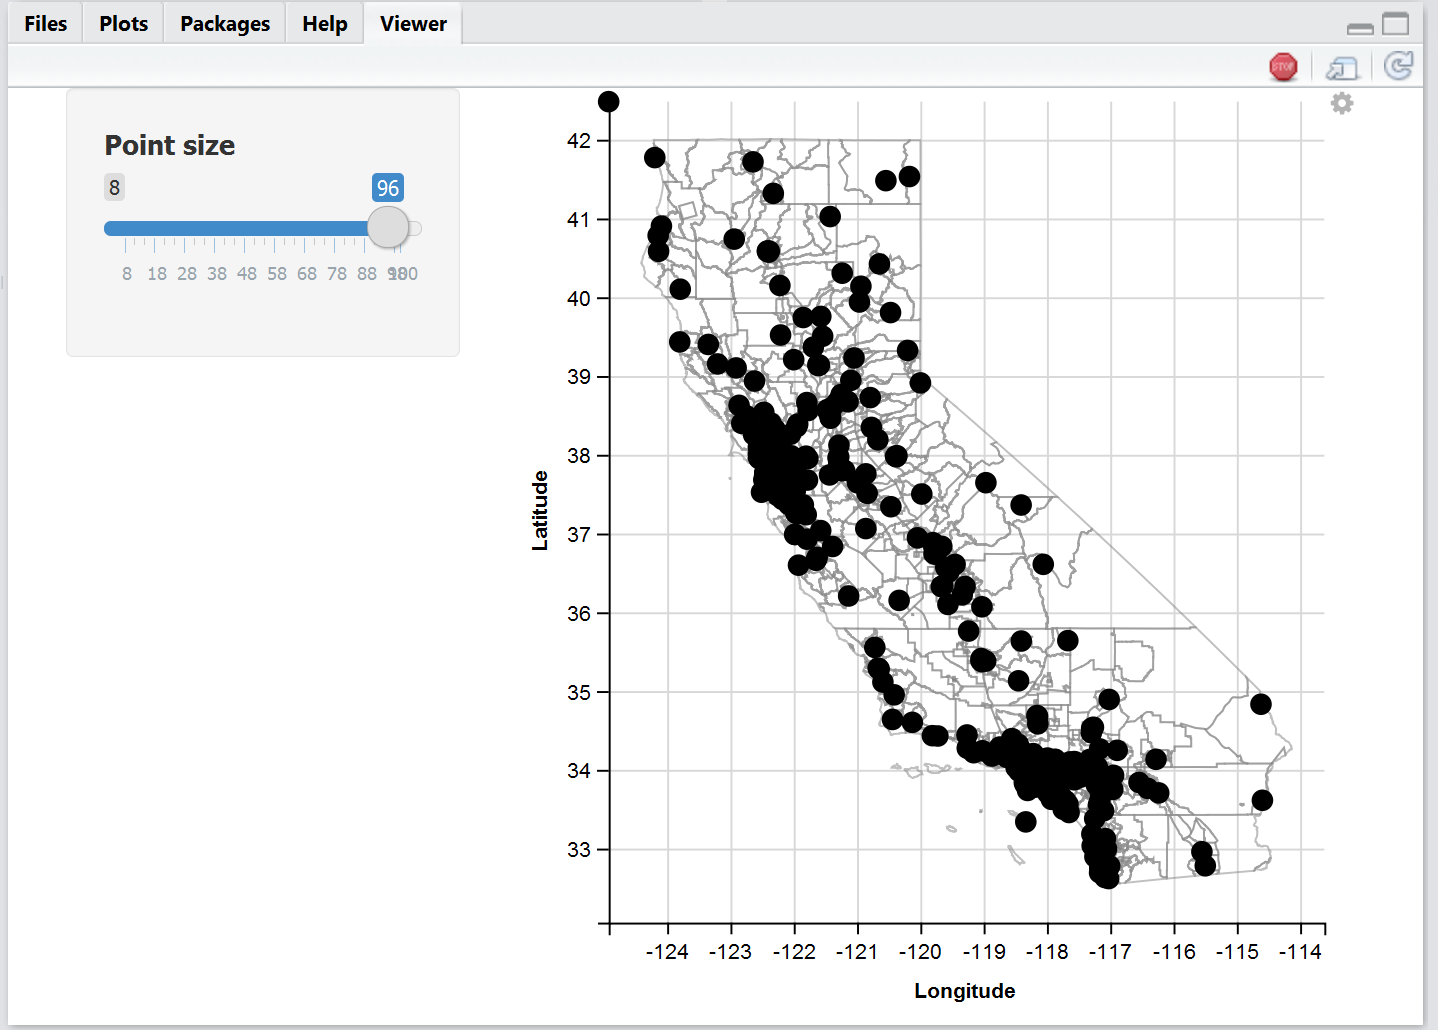
\includegraphics[scale=0.55]{images/shapefile_v3-4-2.png}
  \end{center}

\end{frame}

%---
\subsubsection{Geographical Plots via 'leaflet'}
\begin{frame}[fragile, allowframebreaks]
	\frametitle{Geographical Plots via 'leaflet'}
Another way to make interactive images is via 'leaflet':

\begin{lstlisting}
library(leaflet)
leaflet(data = df_hosp) %>% 
  addTiles() %>%
  addMarkers(
    ~Longitude, 
    ~Latitude, 
    popup = ~as.character(Total.for.Hospital)
    )
\end{lstlisting}

\newpage
  \begin{center}
		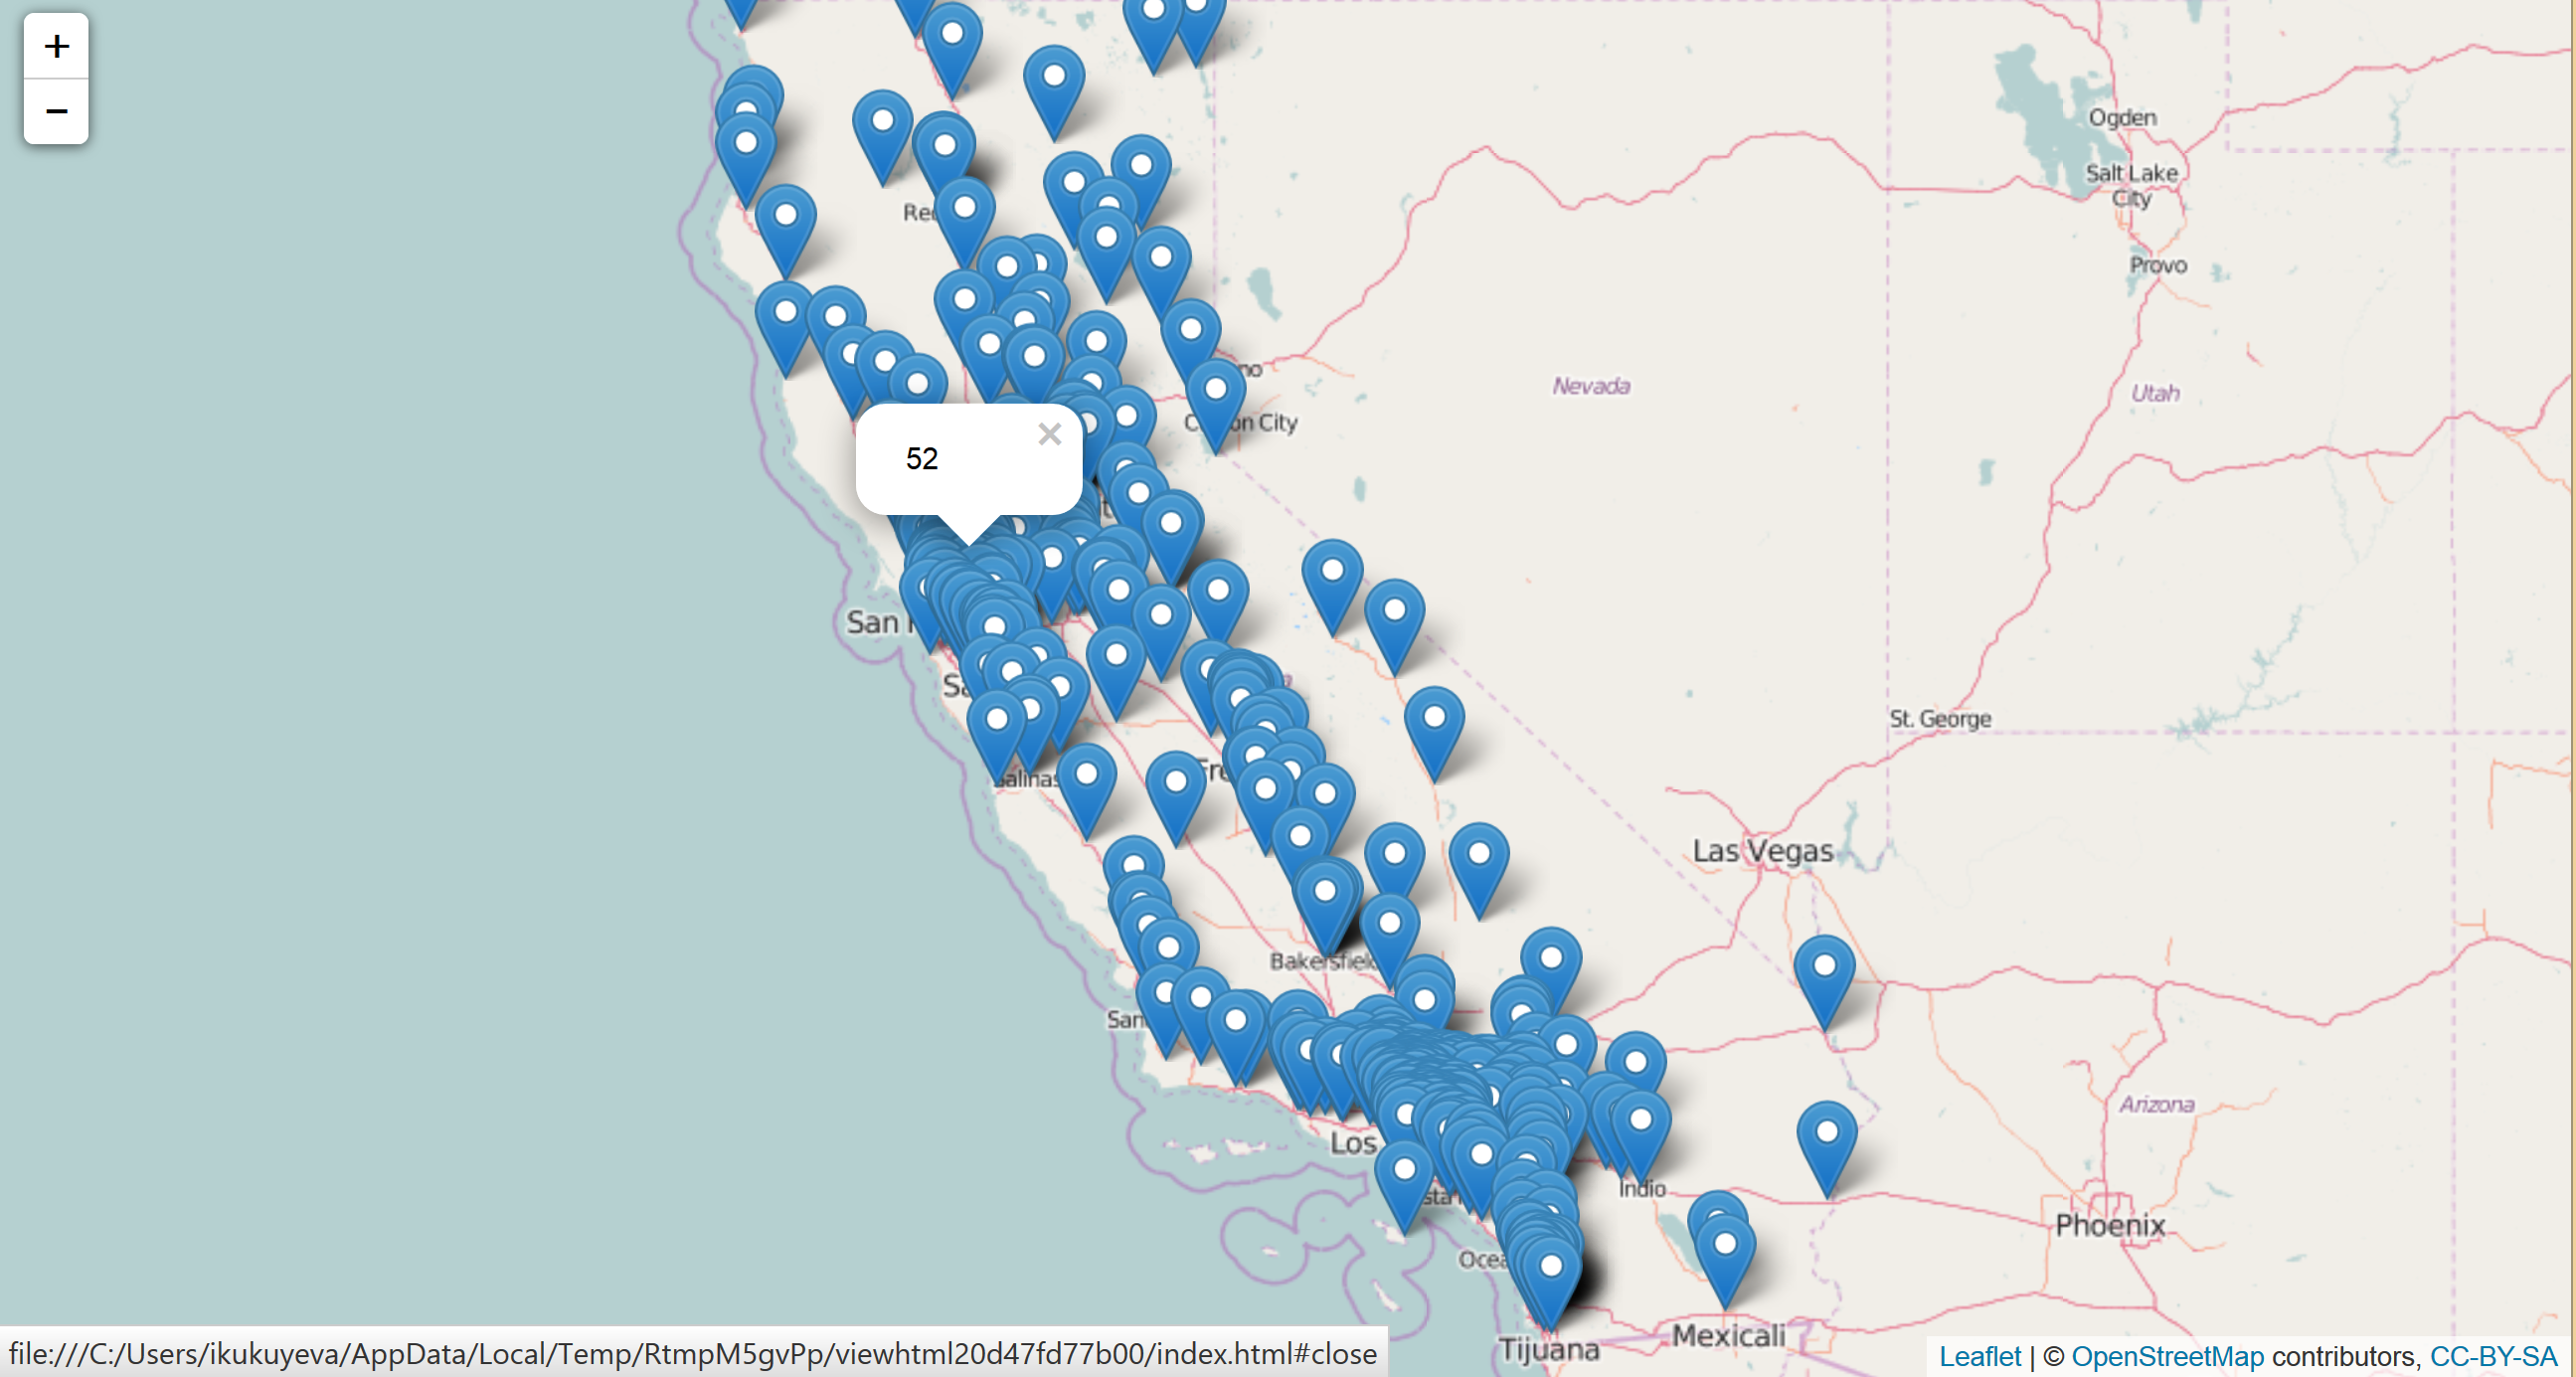
\includegraphics[scale=0.37]{images/leaflet.png}
	\end{center}
\end{frame}

% ------------------------------------------------------------
% ------------------------------------------------------------
\subsection{Exercise III}
\begin{frame}
	\frametitle{Exercise III}
	In the healthcare data set, what's one way to showcase higher volume procedures in the plot?  
\end{frame}
%ozone<-read.table("http://www.ats.ucla.edu/stat/R/faq/ozone.csv", sep=",", header=T)
%attach(ozone)
%plot(Lat~Lon, xlim=c(-125, -113), ylim=c(31,42))
%map("state", "california", add=TRUE)
		% maps +points, bubbleplot
		% locator, identify
		% color-coding for intensity
	
% ------------------------------------------------------------
% ------------------------------------------------------------

%%%%%%%%%%%%%%%%%%%%%%%%%%%%%%%%%%%%%
\section{3D Plots}
\subsection{\ttfamily lattice \normalfont library}
%\begin{frame}
%\frametitle{3D Plots}

%		- lattice, plot3d ...\\
%		- changing plotting options \\
%		- contourplot, wireframe, levelplot \\
%		-rgl, scatterplot3d \\
%		
%\end{frame}

%%%%%%%%%%%%%%%%%%%%%%%
\begin{frame}[fragile]
\title{3D Images}

One way to create 3D images is with the package \ttfamily lattice: \normalfont 

    \begin{columns}
      \column{0.50\textwidth}
\bf{Method 1:} \normalfont Using \ttfamily wireframe(): \normalfont 
\begin{lstlisting}
library(lattice)
wireframe(volcano, color.palette = terrain.colors, asp = 1, color.key=TRUE, drape=TRUE, scales = list(arrows = FALSE))
\end{lstlisting}
%g <- expand.grid(x = 1:10, y = 5:15)
%g$z<-g$x^2
%wireframe(g$z~g$x*g$y, scales = list(arrows = FALSE), drape = TRUE, colorkey = TRUE)

     \column{0.50\textwidth}
       \begin{center}
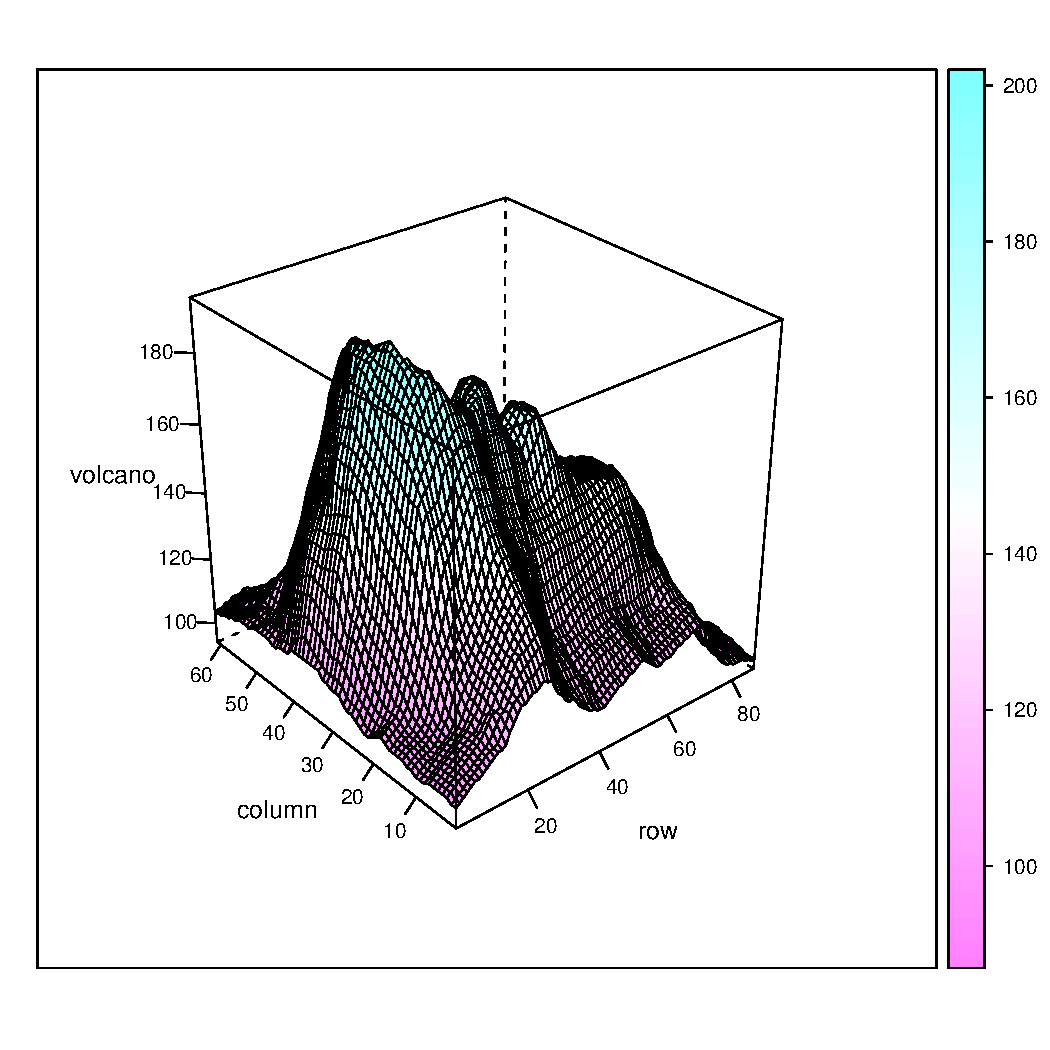
\includegraphics[width = 55mm]{images/wireframe.pdf}
\end{center}
\end{columns}
\end{frame}

%%%%%%%%%%%%%%%%%%%%%%%
\begin{frame}[fragile]
\title{3D Images}

    \begin{columns}
      \column{0.50\textwidth}
\bf{Method 2:} \normalfont Same image with the \ttfamily levelplot(): \normalfont 

\begin{lstlisting}
library(lattice)
levelplot(volcano, color.palette = terrain.colors, asp = 1, color.key=TRUE, drape=TRUE, scales = list(arrows = FALSE))
contour(volcano, add=TRUE, lwd=1.3, labcex=1.3)
\end{lstlisting}

     \column{0.50\textwidth}
       \begin{center}
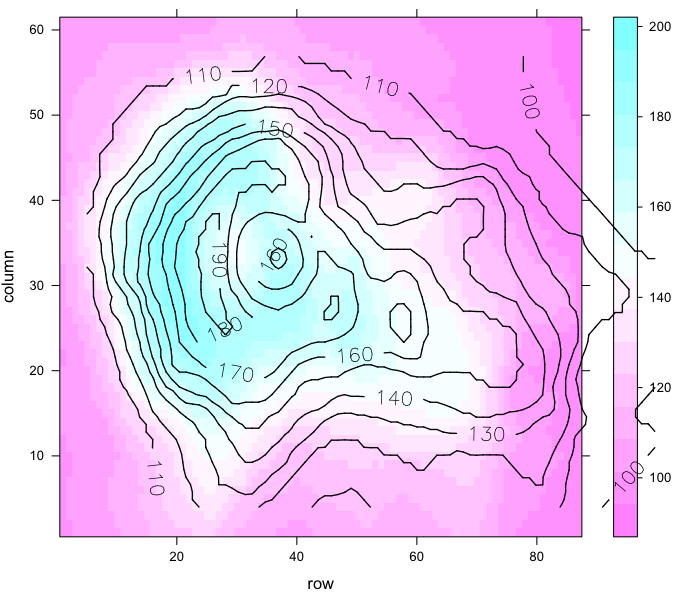
\includegraphics[width = 55mm]{images/levelplot.png}
\end{center}
\end{columns}
\end{frame}
% plot3d(iris)

%%%%%%%%%%%%%%%%%%%%%%%
\subsection{\ttfamily rgl \normalfont library} 
%%%%%%%%%%%%%%%%%%%%%%%
\begin{frame}[fragile]
\title{3D Images}

Another way to create 3D images is with the package \ttfamily rgl: \normalfont 

    \begin{columns}
      \column{0.50\textwidth}
\begin{lstlisting}
library(rgl)
data(quakes)
plot3d(x=quakes[, 2], y=quakes[, 1], z=quakes[, 3], xlab="Longitude", ylab="Latitude", zlab="Depth")
\end{lstlisting}
%g <- expand.grid(x = 1:10, y = 5:15)
%g$z<-g$x^2
%wireframe(g$z~g$x*g$y, scales = list(arrows = FALSE), drape = TRUE, colorkey = TRUE)

     \column{0.50\textwidth}
       \begin{center}
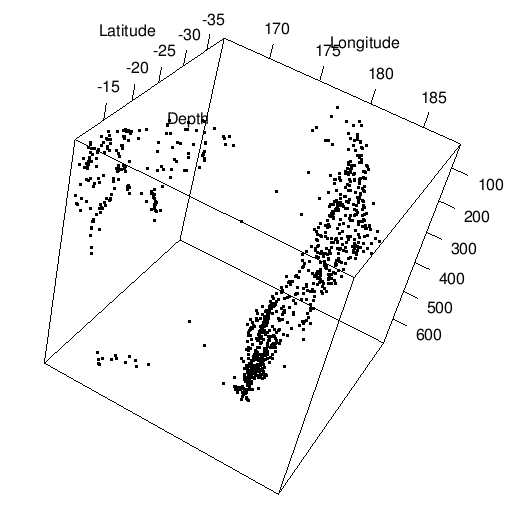
\includegraphics[width = 55mm]{images/Fiji_RGL}
\end{center}
\end{columns}
\end{frame}


% ------------------------------------------------------------
% ------------------------------------------------------------
		
		% lattice, plot3d ...
		% changing plotting options
		% contourplot, wireframe, levelplot	
	%
% ------------------------------------------------------------
% ------------------------------------------------------------

%%%%%%%%%%%%%%%%%%%%%%%%%%%%%%%%%%%%%
\section{Simulation Plots}
\subsection{Preliminaries}
%_______________________

\begin{frame}[fragile]
\frametitle{Simulations}
\framesubtitle{Preliminaries: The function \ttfamily outer() \normalfont}

    \begin{columns}[Tc]
      \column{0.42\textwidth}
\begin{lstlisting}
x=5:6; y=1:3
outer(x,y)
\end{lstlisting}

\begin{beamerboxesrounded}[shadow=true]{}
\ttfamily
\begin{verbatim}
     [,1] [,2] [,3] 
[1,]    5   10   15 
[2,]    6   12   18 
\end{verbatim}
\end{beamerboxesrounded}
\normalfont

	     \column{0.58\textwidth}
\begin{lstlisting}
fcn<-function(x,y){z=x+y}
outer(x,y,fcn)
\end{lstlisting}

\begin{beamerboxesrounded}[shadow=true]{}
\ttfamily
\begin{verbatim}
     [,1] [,2] [,3] 
[1,]    6    7    8 
[2,]    7    8    9 
\end{verbatim}
\end{beamerboxesrounded}
\normalfont
	\end{columns}
\end{frame}

%%%%%%%%%%%%%%%%%%%
\subsection{Performing the Simulation and Visualizing the Results}
%________________________________
\begin{frame}[fragile, allowframebreaks]
\frametitle{Simulations}
\framesubtitle{Visualize with \ttfamily persp() \normalfont}

Suppose we want to know what the function $y\times sin(x)$ looks like:

\begin{lstlisting}
# Sample from the random uniform:
x <- sort(runif(100, min=0, max=10))
y <- x+runif(1)
f <- function(x,y) { r <- y*sin(x)}
z <- outer(x,y,f)
persp(x, y, z, col = "lightblue", shade = 0.1, ticktype = "detailed", expand=0.7)
\end{lstlisting}
% set.seed(04262010)

\newpage
   \begin{figure}[ht]
       \begin{center}
		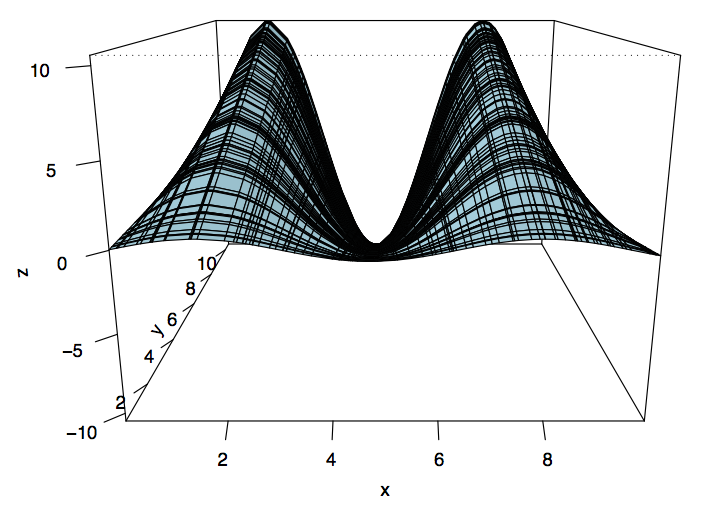
\includegraphics[width = 3.5in]{images/simulation.png}
	\end{center}
   \end{figure}
\end{frame}

%_________
\begin{frame}[fragile, allowframebreaks]
\frametitle{Simulations}
\framesubtitle{Visualize with \ttfamily image() \normalfont}

To visually see its maximum and minimum values, look at the contours of the function:

\begin{lstlisting}
# Format the data appropriate for the image() function:
x.seq<-seq(from=range(x)[1], to=range(x)[2], length=100)
y.seq<-seq(from=range(y)[1], to=range(y)[2], length=100)
n1<-length(x.seq)
n2<-length(y.seq)
mat1<-matrix(z, nrow=n1, ncol=n2, byrow=FALSE)
image(x.seq, y.seq, mat1)
contour(x.seq, y.seq, mat1, add=TRUE)
\end{lstlisting}

\newpage
   \begin{figure}[ht]
       \begin{center}
		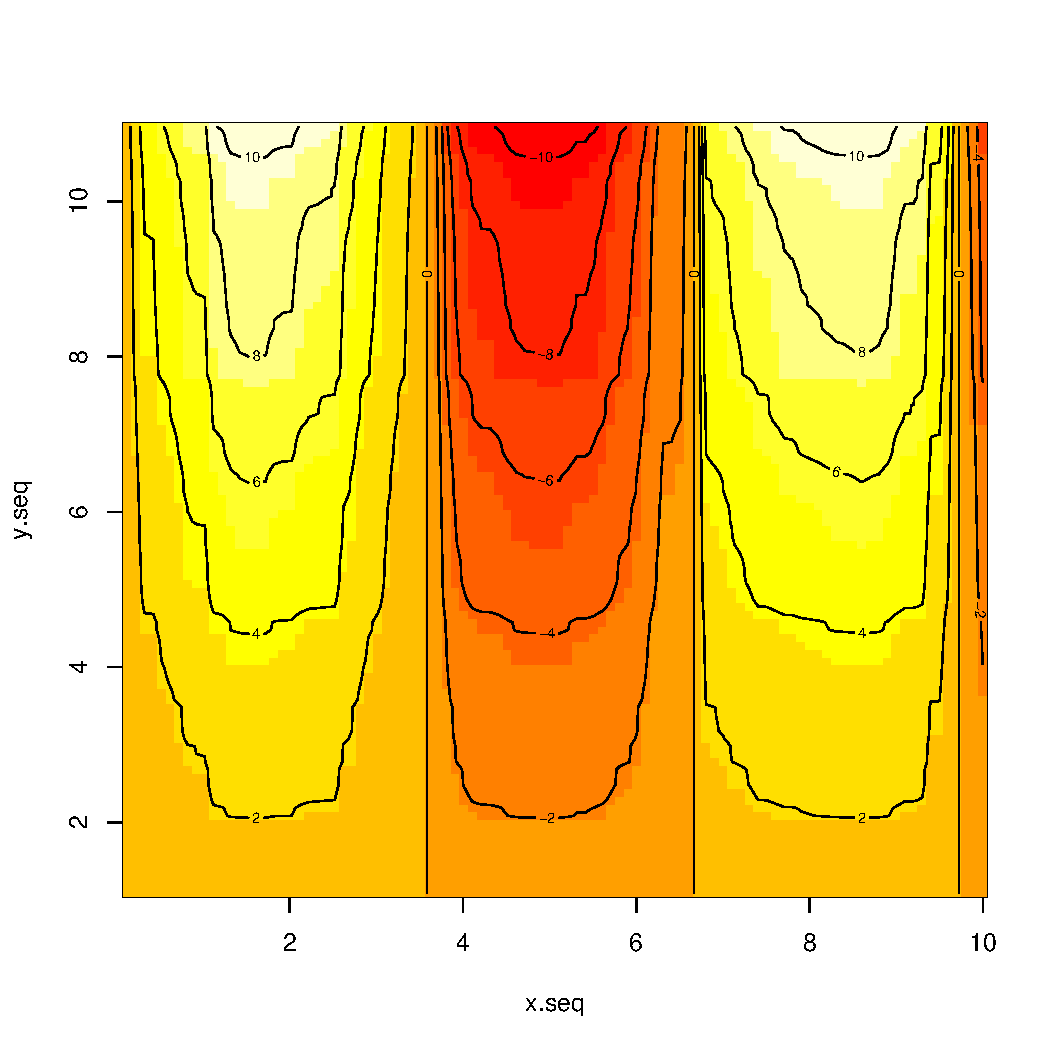
\includegraphics[width = 2.5in]{images/contourSim.pdf}
	\end{center}
   \end{figure}
\end{frame}

%g <- expand.grid(x = 1:10, y = 5:15)
%g$z<-g$x^2
%wireframe(g$z~g$x*g$y, scales = list(arrows = FALSE), drape = TRUE, colorkey = TRUE)

\begin{frame}[fragile, allowframebreaks]
\frametitle{Simulations}
\framesubtitle{Visualize with \ttfamily plot3d() \normalfont}

Suppose we want to know what the function $y\times sin(x)$ looks like with a dynamic plot:

\begin{lstlisting}
# Sample from the random uniform:
x1 <- sort(runif(10000, min=0, max=10))
y1 <- x1+runif(1000, min=0,  max=20)
z1<-y1*sin(x1)
librray(rgl)
plot3d(x1, y1, z1)

\end{lstlisting}

\newpage
   \begin{figure}[ht]
       \begin{center}
		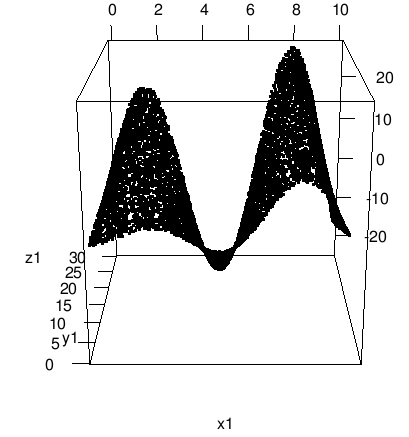
\includegraphics[width = 2in]{images/plot3dSin1.png}
		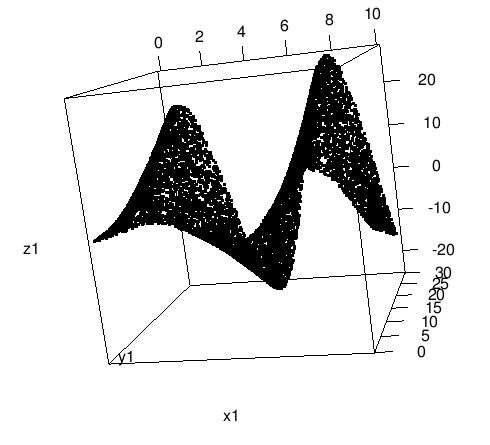
\includegraphics[width = 2in]{images/plot3dSin2.png}
	\end{center}
   \end{figure}
\end{frame}


% ------------------------------------------------------------
% ------------------------------------------------------------
\subsection{Exercise V: Homework Problem}
\begin{frame}
	\frametitle{Exercise V: Homework Problem}
	Visualize the following function:
	\begin{equation}
		z \hspace{0.01in} =\hspace{0.01in} \frac{sin(\frac{3}{2}x)}{y}
	\end{equation}	
\end{frame}

%# Sample from the random uniform:
%x <- sort(runif(100, min=0, max=10))
%y <- x+runif(1)
%f <- function(x,y) { r <- sin(1.5*x)/y}
%z <- outer(x,y,f)
%persp(x, y, z, col = terrain.colors(length(z)/4), shade = 0.1, ticktype = "detailed", expand=0.7)
		% see 202C R Code		
	%%%%%%%%%%%%%%%%%% Section: Exercise
\section[Solutions]{Solutions to the Exercises}
%_______________________ Subsection
  \subsection{Solution to Exercise I}
\begin{frame}[fragile]
  \frametitle{Solution to Exercise I}

			\begin{lstlisting}
beanplot(Sepal.Width ~ Species, data=iris, col=list(grey(0.5),c(grey(0.8),"white")), border = NA, overallline = "median", ll=0.01, side="both")
			\end{lstlisting}
\end{frame}

%_______________________ Subsection
  \subsection{Solution to Exercise II}
  \begin{frame}[fragile]
  \frametitle{Solution to Exercise II}

			\begin{lstlisting}
source("http://www.biostat.jhsph.edu/~rpeng/RR/mvtsplot/mvtsplot.R")		
mvtsplot(EuStockMarkets)
			\end{lstlisting}
\end{frame}

%_______________________ Subsection
  \subsection{Solution to Exercise III}
\begin{frame}[fragile]
  \frametitle{Solution to Exercise III}

			\begin{lstlisting}
ozone<-read.table("http://www.ats.ucla.edu/stat/R/faq/ozone.csv", sep=",", header=T)
attach(ozone)
plot(Lat~Lon, xlim=c(-125, -113), ylim=c(31,42))
map("state", "california", add=TRUE)
			\end{lstlisting}

\end{frame}

%_______________________ Subsection
\subsection{Solution to Exercise IV}
  \begin{frame}[fragile]
  \frametitle{Solution to Exercise IV}
 		\begin{lstlisting}
ozone<-read.table("http://www.ats.ucla.edu/stat/R/faq/ozone.csv", sep=",", header=T)
attach(ozone)
library(rgl)
plot3d(z=Av8top, x=long, y=lat)
 		\end{lstlisting}
\end{frame}

%_______________________ Subsection
\subsection{Solution to Exercise V}
  \begin{frame}[fragile]
  \frametitle{Solution to Exercise V}
 		\begin{lstlisting}
# Sample from the random uniform:
x <- sort(runif(100, min=0, max=10))
y <- x+runif(1)
f <- function(x,y) { r <- sin(1.5*x)/y}
z <- outer(x,y,f)
persp(x, y, z, col = terrain.colors(length(z)/4), shade = 0.1, ticktype = "detailed", expand=0.7)
 		\end{lstlisting}
\end{frame}

	\part{Working with R}
% ------------------------------------------------------------


%%%%%%%%%%%%%%%%%%%%%%%%%%%%%%%%%%%%%
% Section: Software Installation
\section{Installation}
\subsection{Software Installation}
%---
%%%%%%%%%%%%%%%%%%%%%%%
\subsection{Saving Plots as a PDF} 
%%%%%%%%%%%%%%%%%%%%%%%
\begin{frame}[fragile]
\frametitle{Saving Plots as a PDF}
  \framesubtitle{For Static Plots}

  \itshape Note: \normalfont The files will be saved in the folder specified with \ttfamily setwd(). \normalfont
  To save a static plot in \ttfamily R \normalfont as a PDF, use function \ttfamily pdf(): \normalfont

  \begin{lstlisting}
# To save the image to the desktop:
setwd("~/Desktop")
pdf("filename.pdf")
wireframe(volcano, col.regions = terrain.colors(100), asp = 1, color.key=TRUE, drape=TRUE, scales = list(arrows = FALSE))
dev.off()
  \end{lstlisting}

\end{frame}

\begin{frame}[fragile]
  \frametitle{Saving Plots as a PDF}
  \framesubtitle{For Dynamic Plots}

  \itshape Note: \normalfont The files will be saved in the folder specified with \ttfamily setwd(). \normalfont
  To save a dynamic plot in \ttfamily R \normalfont as a PDF, use function \ttfamily rgl.snapshot(): \normalfont

  \begin{lstlisting}
# To save the image to the desktop:
setwd("~/Desktop")
# Step 1: Produce the 3D image:
plot3d(x=quakes$long, y=quakes$lat, z=quakes$depth, xlab="Longitude", ylab="Latitude", zlab="Depth")
# Step 2: Can rotate before taking a snapshot:
rgl.snapshot("quakes.png")
  \end{lstlisting}

\end{frame}

%%%%%%%%%%%%%%%%% 
\section{Common Bugs and Fixes}
%%%%%%%%%%%%%%%%%%%%%%%%%%%%%%%%%%%%%

\subsection{Syntax Error}
\begin{frame}[fragile]
  \frametitle{\ttfamily Error: syntax error \normalfont}
Possible causes:
  \begin{itemize}
    \item Misspelling the object's name
    \item Including a "$+$" when copying code from console/website, etc.
    \item Having an extra parenthesis at the end of a function
    \item Having an extra bracket when subsetting
  \end{itemize}
\end{frame}

\subsection{Trailing $+$}
\begin{frame}[fragile]
  \frametitle{Trailing $+$}
Possible causes:
  \begin{itemize}
    \item Not closing a function call with a parenthesis
    \item Not closing brackets when subsetting
    \item Not closing a function you wrote with a squiggly brace
  \end{itemize}
\end{frame}

\subsection{Error When Performing Operations}
\begin{frame}[fragile]
  \frametitle{\ttfamily Error in ... : requires numeric matrix/vector arguments \normalfont}
Possible causes:
  \begin{enumerate}
    \item Objects are data frames, not matrices
    \item Elements of the vectors are characters \\
  \end{enumerate}
  
Possible solutions:
  \begin{enumerate}
    \item Coerce (a copy of) the data set to be a matrix, with the \ttfamily as.matrix() \normalfont command
    \item Coerce (a copy of) the vector to have numeric entries, with the \ttfamily as.numeric() \normalfont command
  \end{enumerate} 
\end{frame}

\subsection{Error in Calling an Object}
\begin{frame}[fragile]
  \frametitle{\ttfamily Error: ... object not found \normalfont}
Possible causes:
  \begin{enumerate}
    \item Misspelling the object's name
    \item Package containing the object has not been loaded
  \end{enumerate}
  
\end{frame}


%%%%%%%%%%%%%%%%%%%%%%%%%%%%%%%%%%%%%
% Section: R Help
\section[Help]{Getting R Help}
%%%%%%%%%%%%%%%%%%%%%%%%%%%%%%%%%%%%%

\begin{frame}[fragile]
\frametitle{R Help: Approach 1}

  \begin{columns}
  \column{0.4\textwidth}
  For help with any function in R, put a question mark before the function name to determine what arguments to use, examples and background information.

  \begin{lstlisting}
?plot
  \end{lstlisting}

  \column{0.6\textwidth}
    \begin{center}
    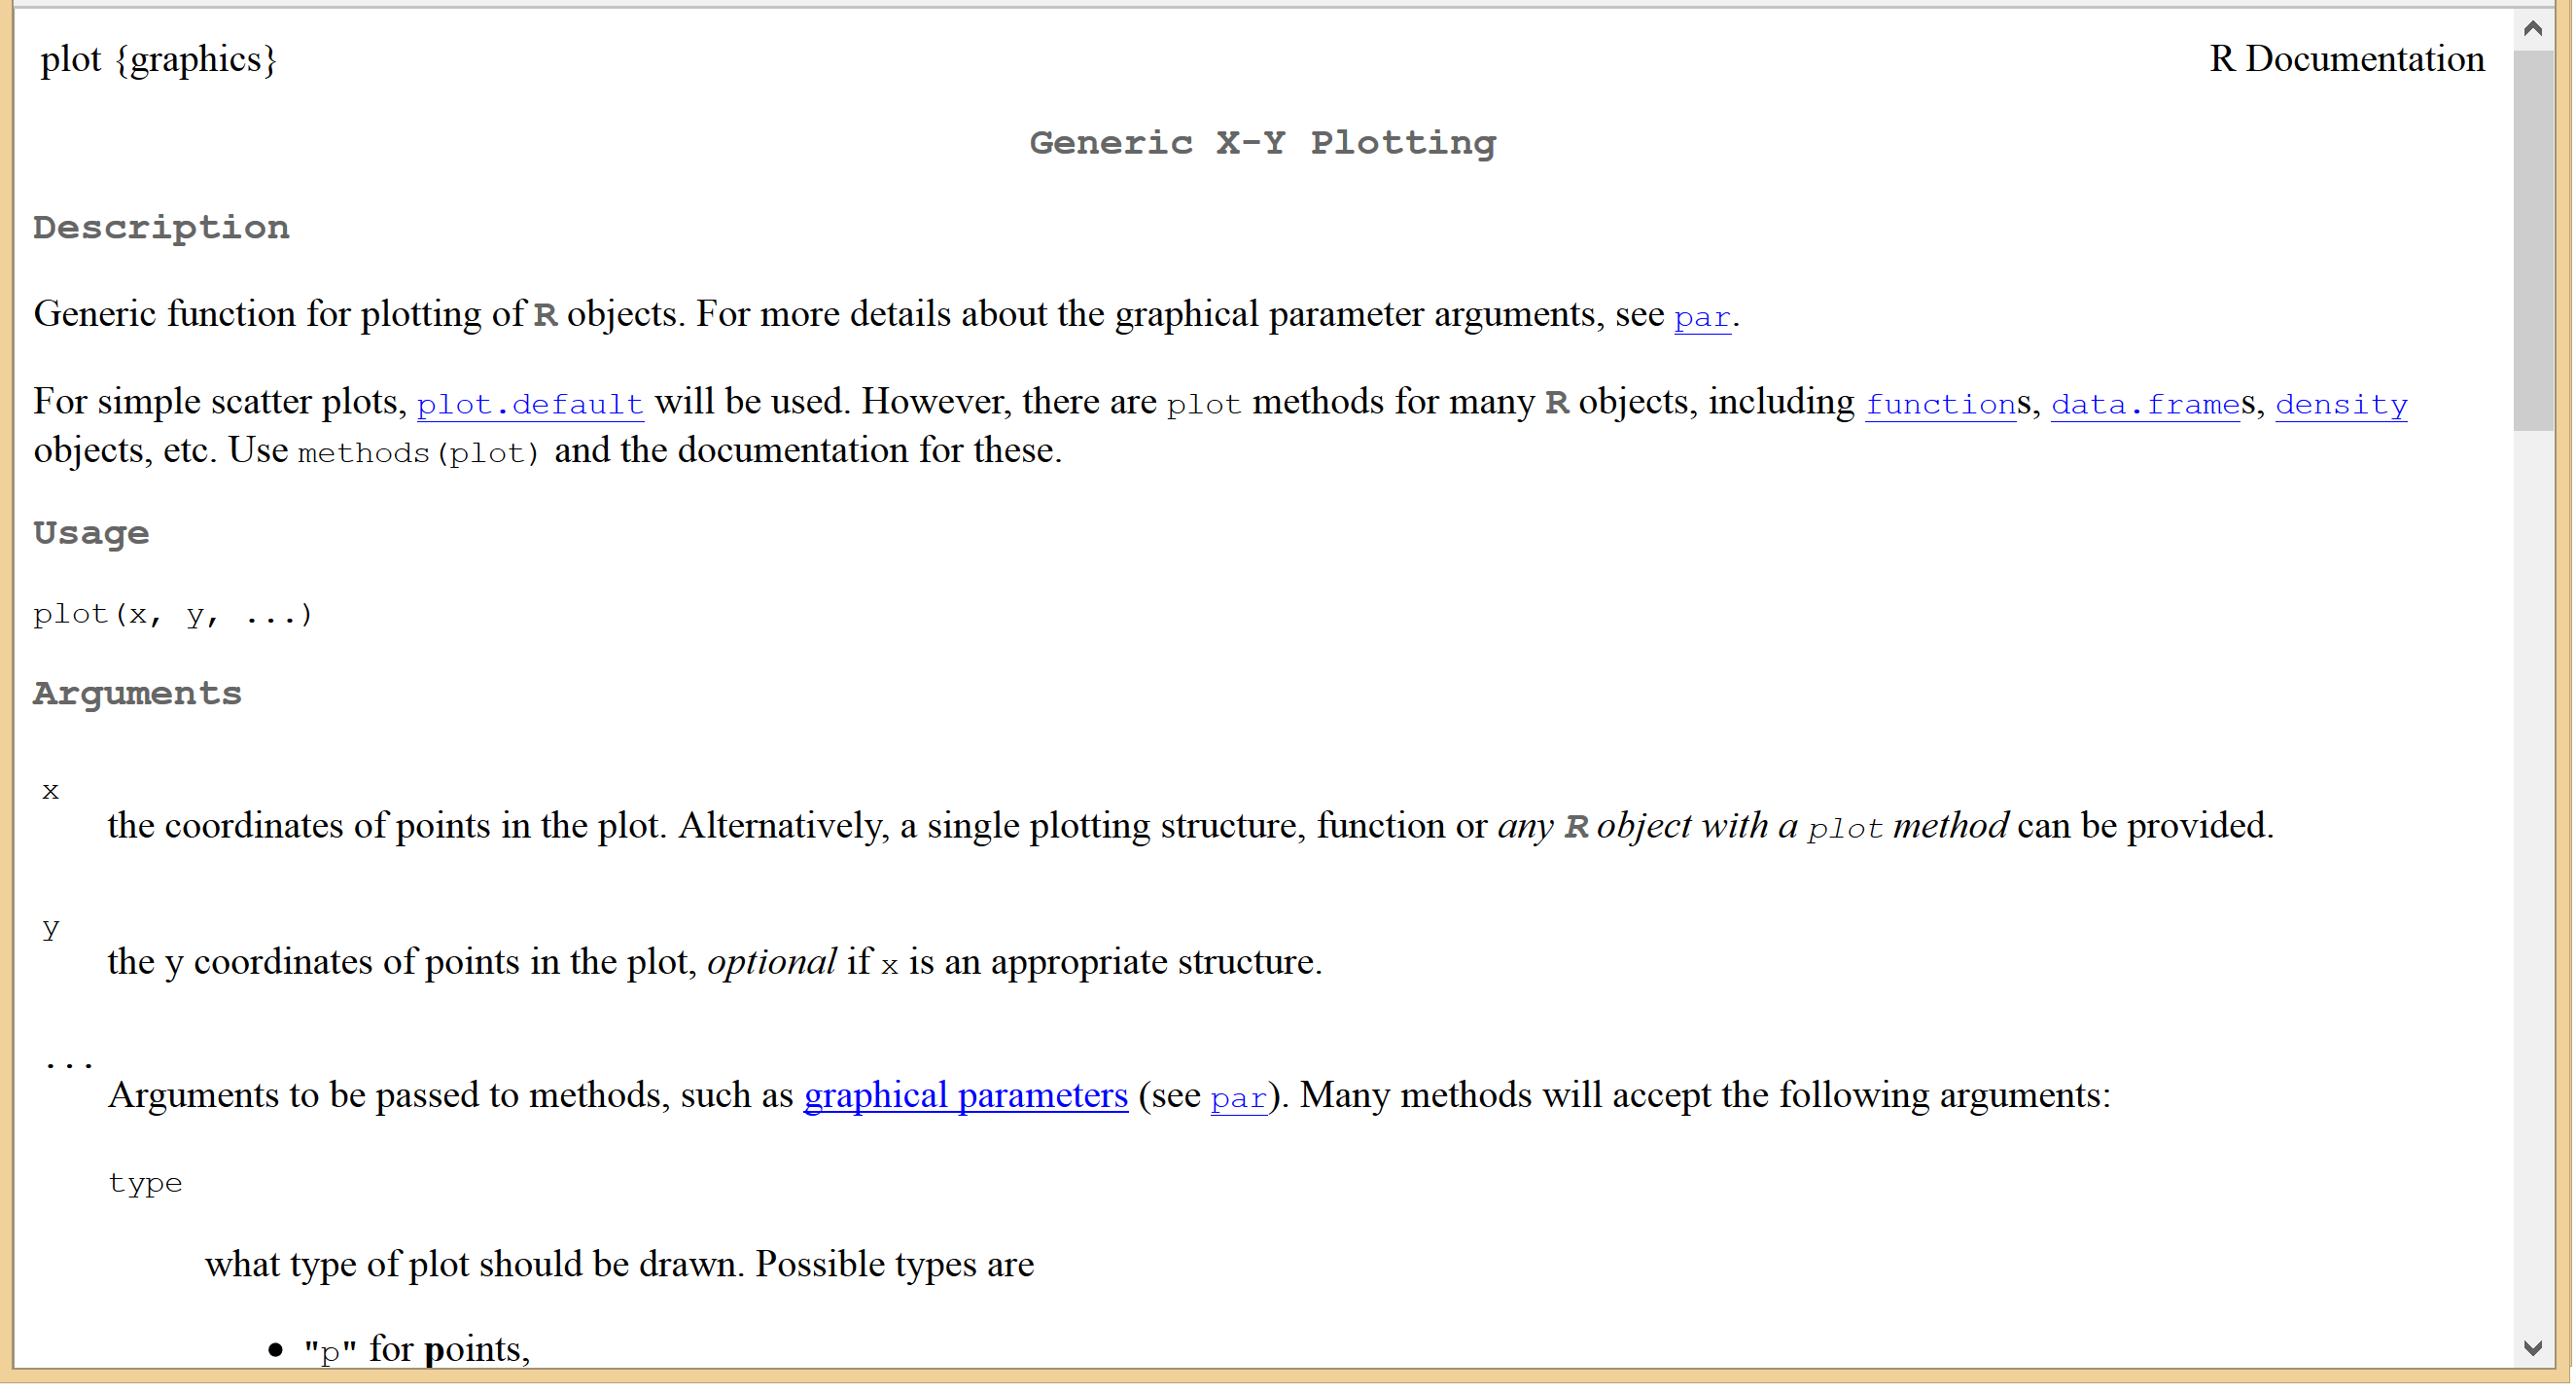
\includegraphics[width=1.1\textwidth]{images/Rhelp}
    \end{center}
  \end{columns}

\end{frame}
%%%---

\begin{frame}[fragile]
\frametitle{R Help: Approaches 2 and 3}

  \begin{columns}
  \column{0.6\textwidth}
  \begin{itemize}
    \item For help with any function in R, search answers on StackOverflow (SO).
    \item For help with any function in R, when all else fails, ask a question on StackOverflow.  Don't forget to follow the SO tips: \url{http://stackoverflow.com/help/how-to-ask}
  \end{itemize}

  \column{0.4\textwidth}
  \begin{center}
  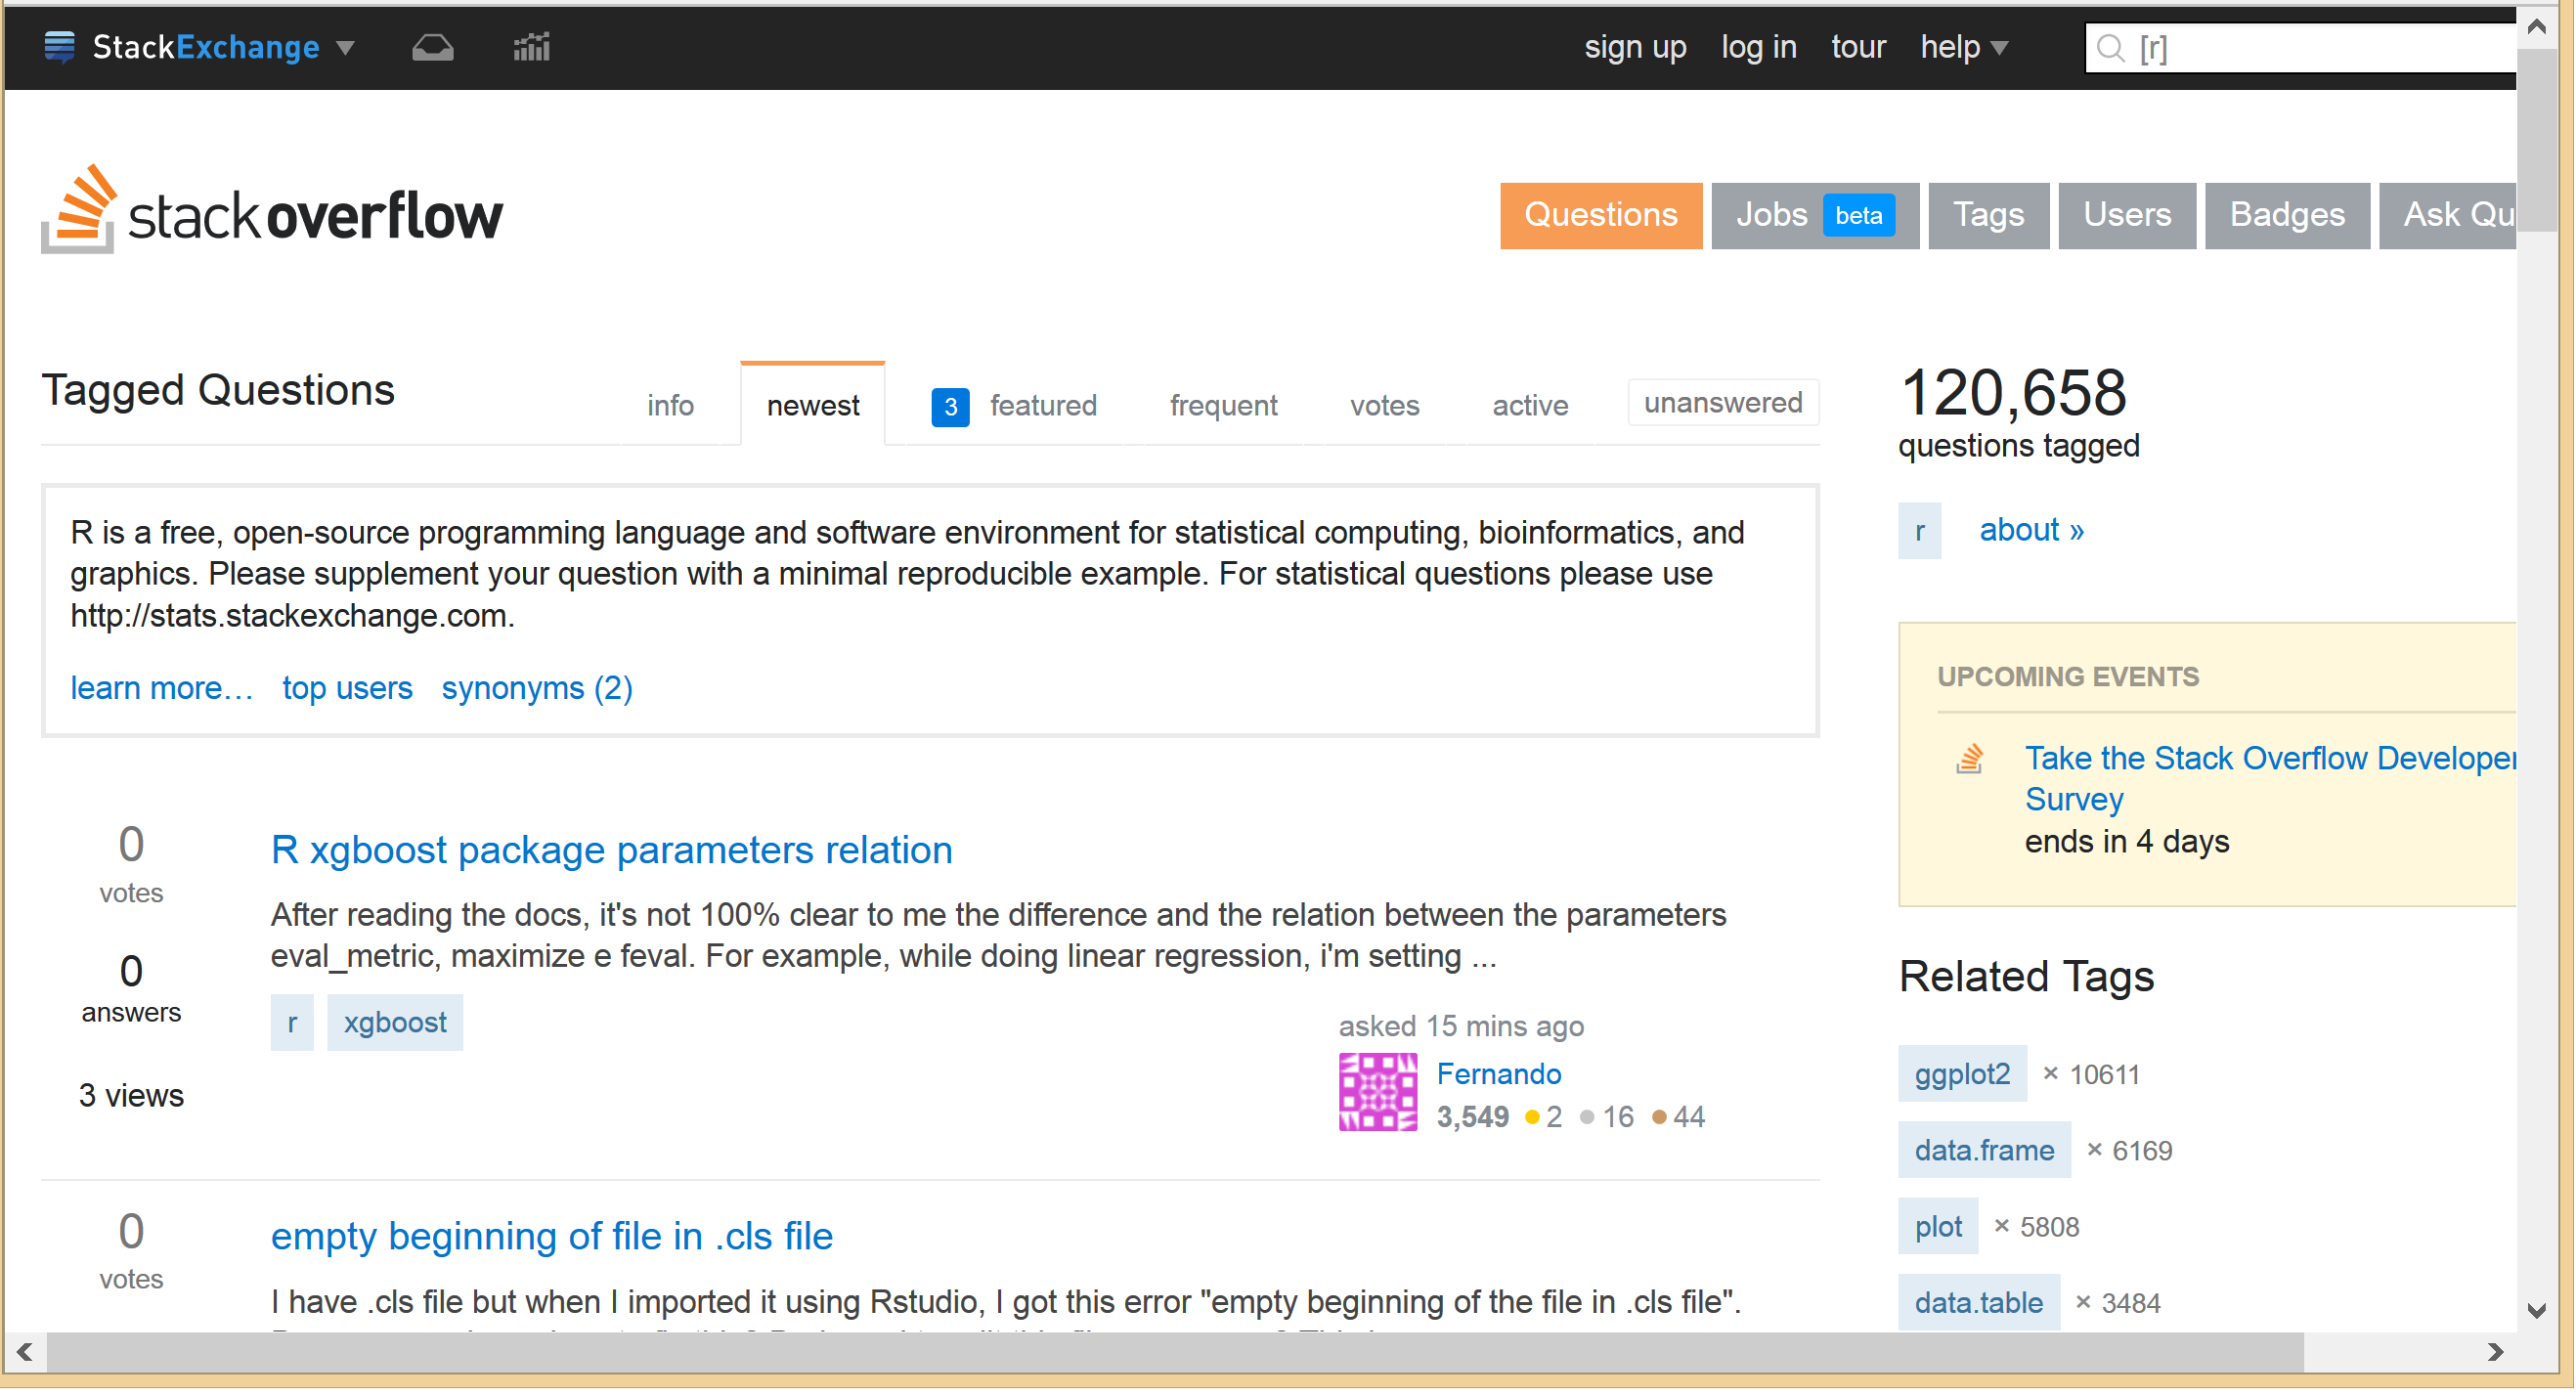
\includegraphics[width=0.95\textwidth]{images/SO}
  \end{center}
  \end{columns}

\end{frame}



%%%%%%%%%%%%%%%%%%%%%%%%%%%%%%%%%%%%%
%--- Online Resources
%%%%%%%%%%%%%%%%%%%%%%%%%%%%%%%%%%%%%
\section[Online Resources]{Online Resources for R}
\begin{frame}[fragile, allowframebreaks]
  \frametitle{Online Resources for R}
%\begin{description}[<+->] 
%\item[Download R:] http://cran.stat.ucla.edu/
%\item[Search Engine for R:] http://rseek.org
%\item[R Reference Card:] http://cran.r-project.org/doc/contrib/Short-refcard.pdf
%\item[UCLA Statistics Information Portal:] http://info.stat.ucla.edu/grad/
%\item[UCLA Statistical Consulting Center:] http://scc.stat.ucla.edu
%\end{description}

\begin{description}
	\item[Download R:] {\small \textit{\urlwofont{http://cran.stat.ucla.edu/}}}
  \item[Download RStudio:] {\small \textit{\urlwofont{https://www.rstudio.com/}}}  
	% \item[Search Engine for R:] {\small \textit{\urlwofont{http://rseek.org}}}
	\item[R Reference Card:] $\:$ \\
		{\small \textit{\urlwofont{http://cran.r-project.org/doc/contrib/Short-refcard.pdf}}}
	\item[R Graphics Gallery:] $\:$ \\
		 {\small \textit{\urlwofont{http://research.stowers-institute.org/efg/R/}}}
	\item[R Graph Gallery:]  {\small \textit{\urlwofont{http://addictedtor.free.fr/graphiques/}}}
	% \item[UCLA Statistics Information Portal:] \small{ \textit{\urlwofont{http://info.stat.ucla.edu/grad/}}}
	% \item[UCLA Statistical Consulting Center:] \small{ \textit{\urlwofont{http://scc.stat.ucla.edu}}}
  \item[] % Book on R graphics: http://book.flowingdata.com/
  \item[More R tutorials:] 
    \begin{itemize}
      \item[]
      \item[IK:] {\small \textit{\urlwofont{http://www.KukuyevaConsulting.com/tutorials}}}
      \item[UCLA IDRE:] {\small \textit{\urlwofont{http://www.ats.ucla.edu/stat/r/}}}
      \item[UCLA SCC:] {\small \textit{\urlwofont{http://scc.stat.ucla.edu/mini-courses/}}}
    \end{itemize}  
  \item[JSS:]
  \item[Stackoverflow:]
  \item[Blogs:]
\end{description}
\end{frame}


% http://adv-r.had.co.nz/ 
% http://www.statmethods.net/interface/packages.html package install
% List of packages https://cran.r-project.org/web/packages/
% Gallery: http://rgraphgallery.blogspot.com/search/label/barchart
% Steam charts: http://www.r-bloggers.com/data-mountains-and-streams-stacked-area-plots-in-r/

%%%%%%%%%%%%%%%%%%%%%%%%%%%%%%%%%%%%%
\section{References}
%%%%%%%%%%%%%%%%%%%%%%%%%%%%%%%%%%%%%

\begin{frame}
  \begin{itemize}
    \item[1.] \url{http://adv-r.had.co.nz/}
    \item[2.] \url{http://www.sixhat.net/how-to-plot-multpile-data-series-with-ggplot.html}
    \item[3.] \url{http://stackoverflow.com/questions/17584248/exact-axis-ticks-and-labels-in-r-lattice-xyplot}
    \item[4.] \url{https://rstudio-pubs-static.s3.amazonaws.com/3364_d1a578f521174152b46b19d0c83cbe7e.html}
    \item[5.] \url{www.jstatsoft.org/v25/c01/paper}
    \item[6.] \url{http://www.kdnuggets.com/2015/05/r-vs-python-data-science.html}
    \item[7.] \url{http://flowingdata.com/2014/02/05/where-people-run/}
    % \item[8.] \url{http://xkcd.com/688/}
    \item[8.] \url{https://www.facebook.com/notes/facebook-engineering/visualizing-friendships/469716398919}
  \end{itemize}
\end{frame}

%_________________________________ Part
%%%%%%%%%%%%%%%%%% Section: Exercise

%\frame{
%  \frametitle{Upcoming Mini-Course}
%	\framesubtitle{This Wednesday}
%$4:30$PM: Advanced Graphics with \ttfamily R \normalfont
%}

\frame{
  \frametitle{}
\begin{center}
Thank you.\\

Any questions?
\end{center}
}

	
%>     -histograms (and overlaying sample and normal densities to it)
%>     -boxplots and adding details
%>     -points plots with different characters and options
%>     -overlaying maps
%>     -creating bubbleplots
%>     -lattice graphics
%>     -3D graphics: scatterplot3d and plot3d
%>     -formatting plots
%>     -saving plots as PDFs, BMP, etc
%>     -creating tables (to be used in LaTeX)
%	
\end{document}
